%\documentclass[journal,onecolumn]{IEEEtran}
\documentclass[11pt, oneside]{article}  
\usepackage{geometry}    
\geometry{letterpaper,margin=1in}       
\usepackage{amsmath} % special symbols
\usepackage{amssymb} % more special symbols
\usepackage{epsfig} % needed for including figures
\usepackage{lipsum} % generate placeholder text
\usepackage[hyphens]{url} % line break URLs
\usepackage{color}
\usepackage{color,soul}
\usepackage[usenames,dvipsnames,svgnames,table]{xcolor} % custom color definition
% \usepackage[figure]{algorithm2e} % advanced written algorithm handling
\usepackage{graphicx} % advanced graphic manipulation handling
\usepackage{epstopdf} % converts vector graphics (eps) to pdf for embedding
\usepackage{longtable} % allows tables to break across multiple pages
\usepackage{makeidx} % create an index
\usepackage{framed}
\usepackage{placeins}
\usepackage{parskip}
\usepackage{enumerate}
\usepackage{cite}
\usepackage{wrapfig}
\usepackage{placeins}
\usepackage{multicol}
\usepackage[T1]{fontenc}
\usepackage[utf8]{inputenc}
\usepackage{tabularx,ragged2e,booktabs,caption}
\usepackage{fancyhdr}
\usepackage{listings}
\usepackage{cases}
\newcolumntype{C}[1]{>{\Centering}m{#1}}
\renewcommand\tabularxcolumn[1]{C{#1}}





% correct bad hyphenation here
\hyphenation{op-tical net-works semi-conduc-tor}


\newcommand{\TODO}[1]{\textcolor{red}{\textbf{TODO: } #1}}


% Yanyu's
\usepackage{cleveref}
\usepackage{algpseudocode}
\usepackage{algorithm}
\algnewcommand\algorithmicinput{\textbf{Input:}}
\algnewcommand\INPUT{\item[\algorithmicinput]}
\algnewcommand\algorithmicoutput{\textbf{Output:}}
\algnewcommand\OUTPUT{\item[\algorithmicoutput]}
\newcommand{\algorithmicbreak}{\textbf{break}}



\begin{document}

\title{\textbf{Identification of Conserved Regions\\ in CRISPR Protein Family}\\ \text{02-712 Final Project}}

% make the title area
\maketitle

\begin{center}
\begin{tabular}{ c c c }
 Christine Baek & Qi Chu & Yanyu Liang \\ 
christib@andrew.cmu.edu & qchu@andrew.cmu.edu & yanyul@andrew.cmu.edu \\     
\end{tabular}\\
\smallskip
\smallskip
Department of Computational Biology, Carnegie Mellon University
\end{center}

\bigskip

% As a general rule, do not put math, special symbols or citations
% in the abstract
\begin{abstract}
In the past few years, CRISPR/\textit{Cas} system has enjoyed exponential growth in terms of studies and applications due to its sequence-level recognition. However, because this is a relatively new topic, while there are many publications demonstrating successful application of \textit{Cas9}, limited studies are currently available on the protein family as a whole. While \textit{Cas9} currently is the CRISPR protein \textit{du jour}, other \textit{Cas} proteins offer much more divergence in terms of PAM sequences, as well as possible reduction in terms of components required and size of the protein complex for \textit{Cas} applications, and could potentially address some of the challenges that have come up in applications of \textit{Cas9}. Therefore, it is imperative that much more studies are done on the \textit{Cas} family as a whole rather than just applications. In this project, we explored the capability of the following three approaches, pairwise sequence alignment, Gibbs Sampling, and HMM profiling, in our attempt to identify conserved regions, or motifs, in the \textit{Cas} family. However, due to limited data and and high divergence of \textit{Cas} proteins, it was proven to be challenging to discover consistent motifs, especially in more complex models but nevertheless offer us insight into CRISPR/\textit{Cas} protein family. 
\end{abstract}



\section{Introduction}
This report explores the evolution and relationship of various \textit{Cas} (CRISPR-associated) proteins. CRISPR is a prokaryotic adaptive immune system that works by base-pair recognition of foreign genetic material and subsequent nuclease activity on the non-self genome. This has been adopted for various applications including genome engineering, and the fact that CRISPR's recognition mechanism based on base-pairing (as opposed to protein-DNA recognition of ZNF or TALENs) result in improved accuracy and reduced costs (no protein engineering involved). CRISPR is as diverse as the species that carry CRISPR in its genome, but ultimately have the same function of adaptive immunity against foreign agents. While \textit{Cas9} (isolated from \textit{Streptococcus pyogenes}) is currently the \text{Cas} protein of choice for such applications due to smallest number of involved components, it would be beneficial to study the other Cas proteins as well, since \textit{s.pyogenes Cas9} is limited in terms of PAM (Protospacer Adjacent Motif), of \texttt{-NGG}), large size of \textit{Cas9} provides limits in some applications, as well as expanding available options for CRISPR engineering. 

\textit{Cas9} currently is predominantly used for genome engineering because it was the first CRISPR protein that was successfully adapted for genome engineering, chosen for its relative simplicity (single gene for all required protein components). In other CRISPR system, the CRISPR functionality is split into multiple \textit{Cas} proteins rather than a single protein, such as in \textit{Cas9}. Now that we know more about the CRISPR system and somewhat better understanding of what each domain does, it may be beneficial to explore using some of the other CRISPR proteins to achieve same goal : use \textit{Cas} protein and its base-pair recognition capacity for various applications ranging from scientific research to genetic therapy. 

\textit{Cas9}'s big size (1368AA residues) has been a source of concern for therapeutic applications.  Prominent delivery tool for \textit{in vivo} and \textit{in vitro} for gene therapy has been adeno-associated virus. While there have been attempts to utilize such delivery method for \textit{Cas9} such as \cite{aav1} or\cite{aav2}, its prohibitively large size has limited number of studies reporting successful gene therapy using both \textit{Cas9} and AAV. Other families of \textit{Cas} proteins are predicted to have different functions split up into multiple genes. As some function of CRISPR system is not necessarily for the purpose of genetic engineering (such as initial cleavage and insertion of foreign genetic material into CRISPR complex), it would be greatly beneficial to identify and isolate specific regions of interest, as well as individual \textit{Cas} proteins that represent those regions, that are directly applicable for genome studies. By identifying conserved motifs between different CRISPR proteins, we can hopefully identify regions of corresponding activity in those CRISPR proteins, and compare to \textit{Cas9} which has been studied in greater detail in terms of structure\cite{cas9structure} or function\cite{mali} compared to other \textit{Cas} proteins. Using other \textit{Cas} proteins would not only allow for greater choice for PAM motifs, but also possibly smaller \textit{Cas} proteins that can accomplish same goals, with less hindrance from the size of protein.

In this report, we employ 3 different approaches to identify motifs, or conserved regions of significance in terms of \textit{Cas} function for better understanding of the \textit{Cas} protein family and mechanism of each component. 

\subsection{CRISPR/Cas} \label{crisprintro}

CRISPR(Clustered regularly interspaced short palindromic repeats) is a microbial adaptive immune system. While bacteria and archaea utilize CRISPR system to store foreign genetic material to distinguish self vs non-self, this system has been adopted and exploited by scientists since 2012 genome engineering tool, as discussed in \cite{jenniferdoudna} and \cite{fengzhang}. CRISPR initially began as next-generation tool to replace ZNFs and TALENs, it has since then been modified for non-genome engineering purposes such as CRISPRi \cite{stanleyqi}. There also have been attempts to reduce off-target effects by modifying the nuclease domain\cite{doublenick} . 

Naturally in bacteria or archaea, CRISPR proteins have distinct roles in the three phases of CRISPR system as follows : 
\begin{enumerate}
\item Acquisition : foreign genetic material enters microbe, which is cut by CRISPR protein and inserted into CRISPR array. This fragment is now a \textit{spacer} separated by \textit{repeats}, hence the name
\item Expression : CRISPR array, which include multiple spacers separated by repeats, is expressed as a single RNA. This is then cleaved into individual units known as \textit{crRNA}, which contain single spacer. \textit{crRNA} forms complex with one or more CRISPR proteins (depending on the CRISPR system)
\item Interference : upon recognition of specific foreign genetic material via base-pairing with the spacer in crRNA, CRISPR protein in complex with the spacer cleaves the foreign genetic material. 
\end{enumerate}



\begin{figure}[ht]
  \centering
  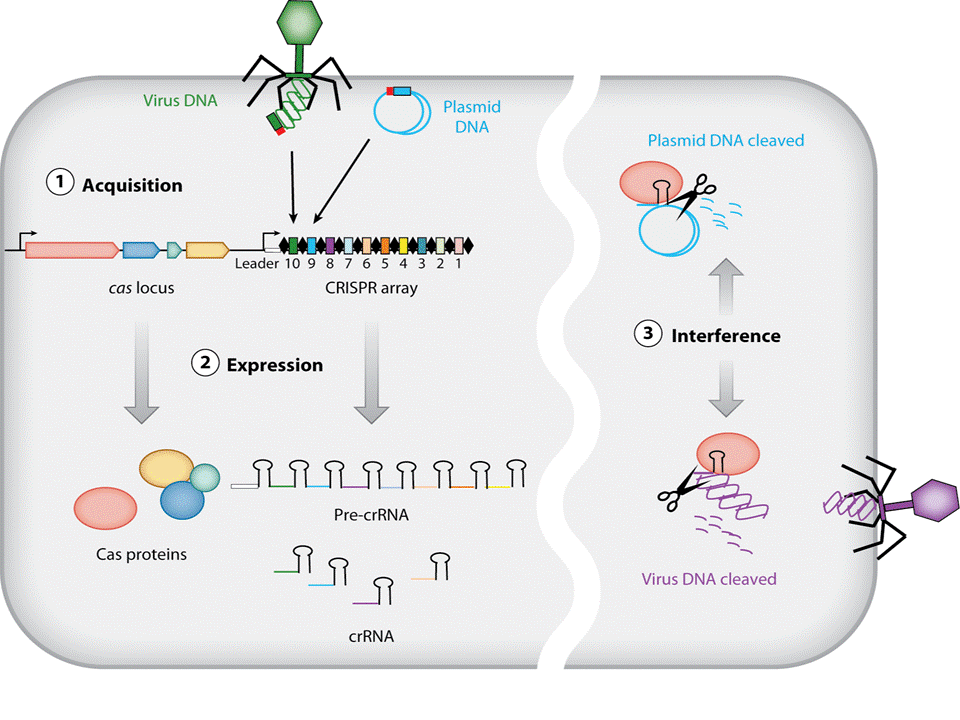
\includegraphics[scale = 0.4]{images/crisprOverview}
      \caption{Overview of CRISPR proteins and their function as described in~\ref{crisprintro} ~\cite{annualreview}}
      \label{crisprOverview}
\end{figure}

\subsection{Past Approaches}
Functionally related regions can be clustered by evidences in experimental data. As summarized in Figure \ref{buildingBlocks}. Previous work has found conserved regions on the sequence level  using sequence alignment and structural information\cite{preWork} inside each sub-type of the \textit{Cas} system but not across the whole \textit{Cas} family.

\begin{figure}[ht]
  \centering
  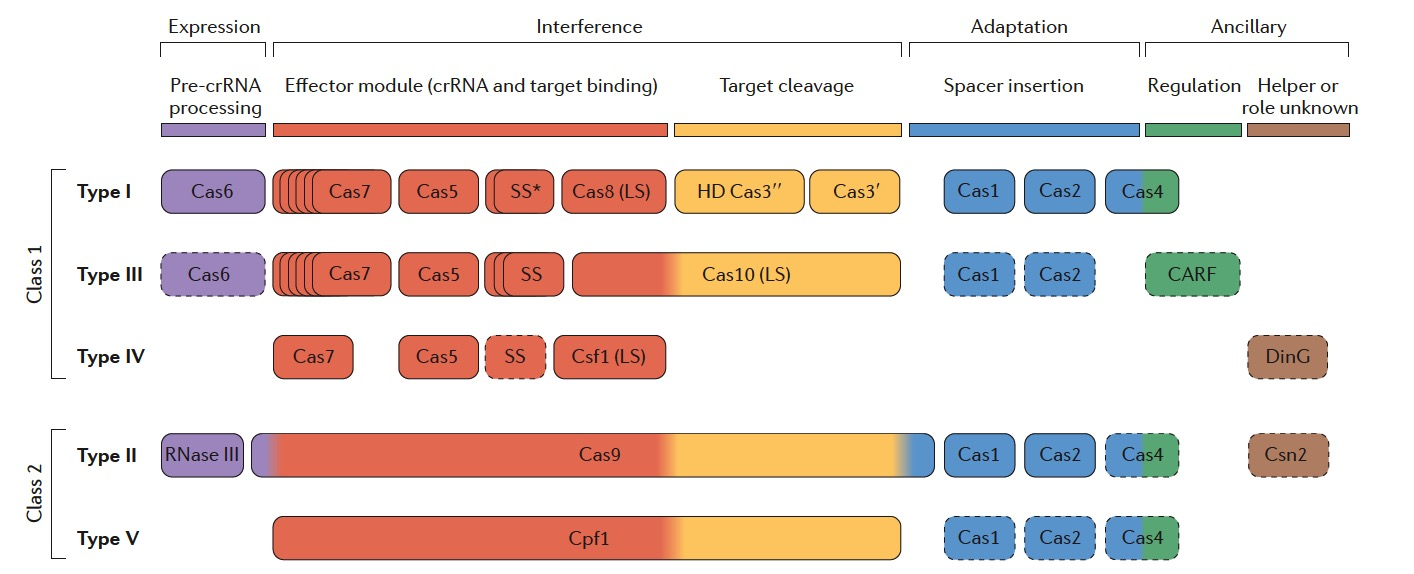
\includegraphics[scale = 0.35]{images/buildingBlocks}
      \caption{Conserved building blocks of \textit{Cas} family proteins \cite{cas:makarova}}
      \label{buildingBlocks}
\end{figure}

\subsection{Goal of Project}

In this paper, we would like to answer the question that whether or not the proteins in Cas family share some sequence level similarity. And more specifically, as Cas9 is a multi-domain protein with multiple functions and each function can be achieved by other single-function protein in Cas family, we would like to explore if we can map such functional domain similarity on the basis of primary sequence similarity between Cas9 and other cas proteins. Informally, we tend to solve the following problem:
\begin{itemize}
	\item \textbf{Input}: Two sets of sequences $C_1 = \{p_1, ..., p_m\}$ and $C_2 = \{q_1, ..., q_n\}$
	\item \textbf{Output}: A set of regions $R = \{r_1, ..., r_k\}$ such that $r_i$ \textit{occurs} and is \textit{representative} in both $C_1$ and $C_2$ 
\end{itemize}
Here \textit{occurs} and \textit{representative} can be explained in different ways under different strategies. In the following section we will discuss the two strategies we proposed to solve this problem.

\subsection{Approaches in This Project}

In this paper, we propose the following two strategies: i) alignment; ii) motif finding. First of all, our problem is naturally a multiple sequence alignment problem. Notice that other Cas proteins is like a substring of Cas9, then to recognize such local similarity, both semi-global alignment and local alignment is suitable in this case. And here \textit{occurs} and \textit{representative} mean that $r_i$ is optimal in alignment.  

Besides profile-based local alignment or semi-global alignment techniques, an alternative approach is to make use of motif information. Motif finding problem is defined as to find representative pattern in a collection of sequences. Following this idea, we can first find motif in $C_1$ and perform pattern recognition in $C_2$. The motif found in $C_1$ carries the \textit{representative} signature of $C_1$ and the recognition in $C_2$ tests whether it meets the requirement to be \textit{occur} in both $C_1$ and $C_2$. Furthermore, for motif analysis, we propose two widely used methods: i) Gibbs sampling; ii) Hidden Markov Models. 

\section{Methods}

All code and output files are available on \texttt{https://github.com/cookie223/CAS\_project}. 

Any reference to files in this report indicate filepath based on root of the repository. 

In this paper, we use 3 different approaches, each with different strengths and limits as for discovering patterns and information from multiple related sequences. Each method has its own section which discusses overview of algorithm/model, pros and cons of given model, detailed protocol and parameters, and analysis performed. 

Protein sequences were used (as opposed to DNA), to uncover preservation of \textit{Cas} protein's functional motifs. Protein sequence analysis much more appropriate for such purpose than DNA sequence especially for distantly related sequences. 

\subsection{Data Retrieval}

Gene sequences for \textit{Cas} family including \textit{Cas1} through \textit{Cas10} were searched and downloaded from NCBI. For each gene, a variety of species were selected to have all the sequences of the proteins in the \textit{Cas} system of one species and also maintain a certain level of variety. The selection is also subject to the availability in NCBI. For domain-specific profile HMM, domain markers were fectched from EMBL-EBI (http://www.ebi.ac.uk). 

\subsection{Sequence Alignment using Dynamic Programming} \label{dpProtocol}

Semiglobal alignment using Needleman-Wunsch\cite{needlemanwunsch} and local alignment using Smith-Waterman Algorithm\cite{smithwaterman} were implemented for pairwise sequence comparison. This is the most intuitive and straight-forward approach for identifying regions of similarity or conserved patterns. However, as simple as the method is, it does have some limitations as discussed in detail below. Because amino acid sequences were used for alignment, it does allow for discrimination between varying degree of conservation or divergence of residues or patterns. While \textit{Cas1, Cas2} and \textit{Cas4} are not part of interference domain and typically not considered in studies for applications of CRISPR/\text{Cas}, I included these proteins in pairwise sequence alignment against \textit{s.pyogenes Cas9} to explore whether there is any sequence similarity within the CRISPR proteins that are currently predicted to be separate genes, and possibly repeated functionality. 



\subsubsection{Model \& Algorithm Overview}

Semiglobal alignment and local alignment were performed on various \textit{Cas} sequences. Because certain families of \textit{Cas} proteins are composed of multiple genes, it is impossible to do a global alignment, or multiple sequence alignment with all \textit{Cas} sequences. Instead, \textit{s.pyogenes Cas9} was used as a reference sequence, to which all other \textit{Cas} sequence was aligned to in pairwise sequence alignment. 

Semiglobal alignment aimed to identify which region of the \textit{Cas} protein as a whole fit to \textit{Cas9}, or the reference sequence (which part of \textit{Cas9} it is most similar to as a whole). As \textit{Cas9} has been studied extensively relative to other \textit{Cas} proteins, this approach aimed to possibly map the function of individual \textit{Cas} protein to a specific region of \textit{Cas9} protein with regions with identified functions. 

Local alignment aimed to identify specific regions that may or may not be smaller than the \textit{Cas} protein itself, compared to \textit{Cas9}. This alignment should be fairly similar in case of highly conserved sequences. However, it may result in \textit{Cas} protein mapping to different regions in \textit{Cas9} depending on the size or the degree of divergence. 

\subsubsection{Pros and Cons}

Because alignment were done against \textit{s.pyogenes Cas9} rather than a progressive alignment, for \textit{Cas} sequences highly divergent from \textit{s.pyogenes Cas9} may be aligned to an inaccurate site. Each alignment is guaranteed to return the global maximum or the most optimal alignment with given parameters, which may or may not be the actual corresponding motif. Also, this method assumes site independence, and does not discriminate conserved regions (which motifs would likely be part of) as opposed to fast-evolving regions. 


\subsubsection{Protocol} 
Following parameters were used for sequence alignment :
\begin{itemize}
\item Scoring Matrix = BLOSUM62 (BLASTP default)
\item Affine Gap Penalty = -10 (BLASTP default is -11)
\item Gap Extension Penalty = -1 (BLASTP default)
\item End Gap Penalty (for Semi-Global only) = -3
\end{itemize}

Gap opening / affine gap penalty was slightly lowered to relax requirement for opening gap, as this experiment is for identifying local regions rather than strict sequence search.


\subsubsection{Analysis}

After each \textit{Cas} sequence was aligned to \textit{s.pyogenes Cas9}, it was then analyzed for the following values :
\begin{itemize}
\item Start position (row, col) of traceback
\item End position (row, col) of traceback
\item Alignment score (based on parameters discussed in section~\ref{dpProtocol}
\item Average Score per base : alignment score / number of bases in alignment
\item \% Sequence Aligned : length of alignment / length of query (non-reference) sequence
\end{itemize}

This was done for both semi-global and local alignment outputs. 

\subsection{Gibbs Sampling}

\subsubsection{Model \& Algorithm Overview}

Gibbs sampling approach is based on position-specific scoring matrix \cite{stormo1982use}, or PSSM, is one of the ways to model a motif. Suppose we are working on sequence set with $\Sigma$ as alphabet and the length of the motif is $w$. Then PSSM is a $|\Sigma|$-by-$w$ matrix with entry:
\begin{align*}
  S_c(A) = \log \frac{\Pr(\text{$A$ is at $c$th column}|\text{motif})}{\Pr(\text{$A$ is at $c$th column}|\text{background})}
\end{align*}
, where $S_c(A), A \in \Sigma$ is the score of alphabet $A$ appearing at $c$th position in the motif and the score is a log odds ratio.

Under PSSM setup, the motif is ungapped with a fixed length and each position is scored independently to each other. PSSM provides a way to parameterize motif and, furthermore, the motif finding problem can be cast as an optimization problem as follow:
\begin{align}
  \max_{S, o} \sum_{i = 1}^n \sum_{c = 1}^w S_c(q_i[o_i + c]) \label{eq:obj}
\end{align}
, where $q_i[x]$ is the $x$th character of $i$th sequence in the collection and $o_i$ indicates the starting site of the motif for $i$th sequence. With various size of the sequence set, this problem is NP-hard and \cite{lawrence1993detecting} has proposed a Gibbs sampling approach to solve it. 

Note that with known $o$, solving for $S$ is reduced to a maximum likelihood estimation, which is trivial to solve, so the core of this problem is to find the optimal $o^{\star}$. Let $S^o$ denote the scoring matrix induced by $o$ and $f_{S}(o)$ denote the objective in \Cref{eq:obj} (with $S$ as scoring matrix), then we can encode the probability distribution of $o$ according to $f(o)$:
\begin{align*}
  \Pr(o) \propto e^{f_{S^o}(o)}
\end{align*} 
Gibbs sampler can be used to sample from this distribution with transition probability as follow:
\begin{align}
  & \log q(o_1, ..., o_i', ..., o_k|o_1, ..., o_i, ..., o_k) \nonumber \\
  =& \log \frac{1}{k}\Pr(o_1, ..., o_i', ..., o_k|o_1, ..., o_i, ..., o_k) \label{eq:exact}\\
  =& S^{(o_1, ..., o_i', ..., o_k)}(o_i')\sum_{j \neq i}^k S^{(o_1, ..., o_i', ..., o_k)}(o_j) + const \nonumber \\
  \approx& S^{o_{-i}}(o_i')\sum_{j \neq i}^k S^{o_{-i}}(o_j) + const \nonumber \\
  =& S^{o_{-i}}(o_i') + const \label{eq:approx}
\end{align} 
, where $S^{o_{-i}}$ is the scoring matrix derived from $o$ without $o_i$ and $S(o_i)$ is the score of $o_i$ based on $S$. With this setup, \cite{lawrence1993detecting} proposed \Cref{algo:gibbs}.
\begin{algorithm}
  \caption{Gibbs sampler for motif finding}
  \label{algo:gibbs}
  \begin{algorithmic}[1]
    \INPUT{sequence set $q$, motif width $w$}
    \OUTPUT{set of starting points $o$}
    \State initialize $o$
    \State $o^{\star} \leftarrow o$
    \While{forever}
      \State pick $i$ from $1, ..., |q|$ with uniform distribution
      \State update $S \leftarrow S^{o_{-i}}$
      \State compute transition probability $p(o_i') \leftarrow \exp\{S(o_i')\}$
      \State update $o_i \sim \text{Multinomial}(p, 1)$
      \State update $o^{\star}$ if there is any improvement
    \EndWhile
  \end{algorithmic}
\end{algorithm}

\subsubsection{Pros and Cons}

Gibbs sampling approach is easy to implement and it converges to optimal solution as the running time goes to infinity. Besides, PSSM representation of a motif is easy to understand and visualize. While, the downside of this approach is that it cannot bear gap. If the sequence collection shares a gapped motif, PSSM based Gibbs sampler will fail to recognize it. Furthermore, the length of the motif and the number of steps are two hyper-parameters which should be specified by the user. In practice, it takes extra computing time to search for a suitable width and to stop early or later is instance specific, and has no general strategy to follow.

\subsubsection{Protocol}

Following steps were applied to the analysis:
\begin{enumerate}
	\item Implement a Gibbs sampler described in \Cref{algo:gibbs}
	\item Train a set of motifs with various widths using Cas5 and Cas7
	\item Score Cas9 sequences based on learned motifs
\end{enumerate}
The widths used started from 10 to up to 190 and the size of interval was 10. To retrieve not only the most representative motif but other sub-optimal ones, for every width we repeated the Gibbs sampling procedure five times and recorded the best output for every run. For every Markov chain, we ran 600 steps because it was sufficient to reach a suboptimal with 600 steps for all instances in analysis.

\subsubsection{Analysis}
To show our Gibbs sampler converge, we track the objective value along the Markov chain. And to show our motif finding based strategy works, we performed the proposed procedure on simulated sequences and globin sequences given in Hmmer\cite{hmmer} where two sets of sequences share similar primary sequence patterns and checked whether our approach could recover such similarity.

\subsection{Domain-specific profile HMM}

\subsubsection{Model \& Algorithm Overview}
To find out whether a sequence of amino acid belongs some domain, we can build a model of the domain and try to match the sequence of the model. Profile Hidden Markov Model is one of the 
models we can build to figure out whether a sequence contains the domain. The model of profile HMM is shown in Figure \ref{HMM}. 

\begin{figure}[ht]
  \centering
  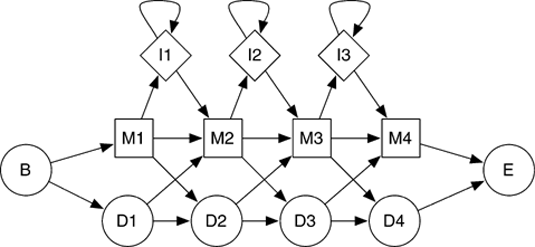
\includegraphics[scale = 0.7]{images/profileHMM}
      \caption{Profile Hidden Markov Model\cite{hmmer}}
      \label{HMM}
\end{figure}


\subsubsection{Pros and Cons}
\begin{itemize}
\item Pros
\begin{enumerate}
\item We can leverage the abundant prior knowledge of Cas9 domain markers by building profile HMM using the alignment of the domains rather than the full sequence.
\item Compared with pair-wise sequence alignment, HMM can find more cases of distantly related sequences.
\item As shown in the figure, HMM can model insertions and deletions.
\end{enumerate}
\item Cons
\begin{enumerate}
\item To leverage the prior knowledge of domain markers, those markers need to be fetched separately from other data source rather than learned by the algorithm.
\item The number of parameters is very large and they need to be optimized.
\end{enumerate}
\end{itemize}


\subsubsection{Protocol}
\begin{enumerate}[a.]
\item A set of \textit{Cas9} or \textit{Cas5} sequences and their domain markers are fetched from EMBL-EBI (http://www.ebi.ac.uk).
\item Sequences of each of the shared domains are subtracted from the full \textit{Cas9} or \textit{Cas5} sequences.
\item For each domain, multiple sequences from different \textit{Cas9} or \textit{Cas5} are aligned by Clustal Omega (http://www.clustal.org/).
\item  A profile HMM is built on the multiple sequence alignment for each domain by Hmmer (http://hmmer.org/)\cite{hmmer}.
\item Search for matches using the profile HMM in the sequences of all previously downloaded \textit{Cas} family proteins.
\end{enumerate}


\subsubsection{Analysis}
For method testing, a set of globin sequences given in Hmmer\cite{hmmer} is used. Since there are \textit{Cas9} and \textit{Cas5} in the previously downloaded \textit{Cas} family proteins sequences, they also act as positive control since the method should be able to find the domains in these proteins.\\
For output analysis, HMM is able to give the probability of given sequence emitted from the underlying domain profile HMM.





\section{Results}

Each of the three approaches for identifying motifs of \textit{Cas} proteins and the resulting data are presented below. 


\subsection{Sequence Alignment using Dynamic Programming}

\begin{minipage}{\linewidth}
\smallskip
\centering
\captionof{table}{Semi-Global Alignment Output} \label{sgoutput} 
\begin{tabular}{ p{1.25in} C{.85in} *4{C{.75in}}}\toprule[1.5pt]
\bf Gene Name & \bf Alignment Score & \bf Average Score / base & \bf \% Sequence aligned & \bf Traceback Start & \bf Traceback End\\\midrule
Cas10\_Mtuberculosis & 234 & 0.212148685 & 1 & [1365][810] & [330][1]\\ 
Cas10\_Phorikoshii & 335 & 0.249813572 & 1 & [1368][762] & [41][1]\\ 
Cas10\_Ssolfataricus & 364 & 0.27063197 & 1 & [1322][1046] & [62][1]\\ 
Cas10\_Tvolcanium & 343 & 0.305976806 & 1 & [1203][776] & [146][1]\\ 
Cas1\_DvsH\_plasmid & 160 & 0.282186949 & 1 & [1297][344] & [734][1]\\ 
Cas1\_Gvaginalis & 163 & 0.332653061 & 1 & [1367][321] & [886][1]\\ 
Cas1\_K-12 & 105 & 0.243055556 & 0.911764706 & [428][306] & [1][28]\\ 
Cas1\_Tdenticola & 176 & 0.387665198 & 1 & [519][291] & [79][1]\\ 
Cas2\_K-12 & 65 & 0.5 & 1 & [528][95] & [400][1]\\ 
Cas2\_Lsalivarius & 64 & 0.444444444 & 1 & [617][102] & [476][1]\\ 
Cas2\_StB20-like & 68 & 0.586206897 & 1 & [217][88] & [102][1]\\ 
Cas3\_DvsH\_plasmid & 152 & 0.145315488 & 1 & [1059][703] & [32][1]\\ 
Cas3\_Gvaginalis & 260 & 0.229681979 & 0.858199753 & [1119][811] & [1][116]\\ 
Cas3\_K-12 & 233 & 0.185805423 & 1 & [1254][889] & [29][1]\\ 
Cas4\_K-12 & 171 & 0.341317365 & 1 & [1323][364] & [833][1]\\ 
Cas4\_Ssolfataricus & 87 & 0.294915254 & 1 & [679][203] & [387][1]\\ 
Cas4\_TtenaxKra & 57 & 0.230769231 & 1 & [573][191] & [330][1]\\ 
Cas5\_Gvaginalis & 140 & 0.309050773 & 1 & [1185][292] & [733][1]\\ 
Cas5\_K-12 & 79 & 0.302681992 & 0.8 & [261][225] & [1][46]\\ 
Cas6\_Cbotulinum & 158 & 0.478787879 & 1 & [740][230] & [414][1]\\ 
Cas6\_Hvolcanii\_plasmid & 99 & 0.25848564 & 1 & [1309][273] & [929][1]\\ 
Cas6\_Ssolfataricus & 118 & 0.280952381 & 1 & [1117][288] & [701][1]\\ 
Cas7\_Hvolcanii\_plasmid & 164 & 0.316602317 & 1 & [899][341] & [390][1]\\ 
Cas7\_K-12 & 171 & 0.341317365 & 1 & [1323][364] & [833][1]\\ 
Cas7\_Ssolfataricus & 147 & 0.267272727 & 1 & [950][312] & [404][1]\\ 
Cas8\_LsV & 136 & 0.265625 & 1 & [1289][314] & [783][1]\\ 
Cas8\_Pdistasois & 237 & 0.295511222 & 1 & [1342][573] & [559][1]\\ 
Cas8\_Pgingivalis & 212 & 0.280794702 & 1 & [1340][500] & [609][1]\\ 
Cas9\_Bthermosphacta & 1726 & 1.249818972 & 1 & [1365][1301] & [47][1]\\ 
Cas9\_Cindologenes & 476 & 0.282157676 & 1 & [1366][1444] & [3][1]\\ 
Cas9\_Cochracea & 375 & 0.276344878 & 0.650315347 & [1322][1427] & [1][500]\\ 
Cas9\_Hpullorum & 180 & 0.27820711 & 1 & [643][345] & [4][1]\\ 
Cas9\_Hpullorum\_2 & 330 & 0.391459075 & 1 & [1347][703] & [549][1]\\ 
Cas9\_Kkingae & 520 & 0.370634355 & 0.997172479 & [1341][1061] & [1][4]\\ 
Cas9\_Movipneumoniae & 519 & 0.340998686 & 0.988216811 & [1349][1273] & [1][16]\\ 
Cas9\_Nlactamica & 505 & 0.353889278 & 0.994459834 & [1368][1083] & [1][7]\\ 
Cas9\_Pacidlactici & 1786 & 1.209207854 & 0.999267399 & [1366][1365] & [1][2]\\ 
Cas9\_Pnultocida & 510 & 0.365068003 & 0.997161779 & [1348][1057] & [1][4]\\ 
Cas9\_Ranatipestifer & 391 & 0.239143731 & 1 & [1366][1406] & [3][1]\\ 
Cas9\_Sgallolyticus & 4529 & 3.274765004 & 0.999271137 & [1368][1372] & [1][2]\\ 
Cas9\_Smoniliformis & 514 & 0.327597196 & 1 & [1368][1260] & [3][1]\\ 
Cas9\_Spaucimobilis & 415 & 0.290616246 & 1 & [1362][1091] & [3][1]\\
\bottomrule[1.25pt]
\end {tabular}\par
\bigskip
Method as discussed in section~\ref{dpProtocol}. Visualization of data is available in Figure~\ref{dp1}
\end{minipage}

\begin{minipage}{\linewidth}
\smallskip
\centering
\captionof{table}{Local Alignment Output} \label{locoutput} 
\begin{tabular}{ p{1.25in} C{.85in} *4{C{.75in}}}\toprule[1.5pt]
\bf Gene Name & \bf Alignment Score & \bf Average Score / base & \bf \% Sequence aligned & \bf Traceback Start & \bf Traceback End\\\midrule
Cas10\_Mtuberculosis & 317 & 0.239064857 & 0.988888889 & [1345][808] & [46][8]\\ 
Cas10\_Phorikoshii & 313 & 0.246650906 & 0.874015748 & [1368][705] & [105][40]\\ 
Cas10\_Ssolfataricus & 432 & 0.316020483 & 0.864244742 & [1365][929] & [16][26]\\ 
Cas10\_Tvolcanium & 362 & 0.312878133 & 0.923969072 & [1312][749] & [165][33]\\ 
Cas1\_DvsH\_plasmid & 152 & 0.290630975 & 0.959302326 & [1237][342] & [728][13]\\ 
Cas1\_Gvaginalis & 120 & 0.270880361 & 0.99376947 & [1332][320] & [904][2]\\ 
Cas1\_K-12 & 107 & 0.29558011 & 0.666666667 & [1340][263] & [983][60]\\ 
Cas1\_Tdenticola & 124 & 0.294536817 & 0.965635739 & [1096][287] & [687][7]\\ 
Cas2\_K-12 & 43 & 0.651515152 & 0.663157895 & [1119][86] & [1055][24]\\ 
Cas2\_Lsalivarius & 77 & 0.611111111 & 0.794117647 & [621][101] & [496][21]\\ 
Cas2\_StB20-like & 72 & 1.028571429 & 0.568181818 & [738][87] & [669][38]\\ 
Cas3\_DvsH\_plasmid & 210 & 0.195712954 & 0.944523471 & [1099][683] & [48][20]\\ 
Cas3\_Gvaginalis & 261 & 0.244382022 & 0.937114673 & [1317][790] & [272][31]\\ 
Cas3\_K-12 & 248 & 0.245787909 & 0.750281215 & [1232][873] & [265][207]\\ 
Cas4\_K-12 & 177 & 0.353293413 & 0.848901099 & [1355][325] & [856][17]\\ 
Cas4\_Ssolfataricus & 100 & 0.304878049 & 0.827586207 & [1308][180] & [981][13]\\ 
Cas4\_TtenaxKra & 60 & 0.810810811 & 0.277486911 & [883][175] & [811][123]\\ 
Cas5\_Gvaginalis & 159 & 0.42513369 & 0.863013699 & [797][274] & [424][23]\\ 
Cas5\_K-12 & 77 & 0.292775665 & 0.68 & [493][184] & [233][32]\\ 
Cas6\_Cbotulinum & 132 & 0.371830986 & 0.82173913 & [453][215] & [99][27]\\ 
Cas6\_Hvolcanii\_plasmid & 93 & 0.322916667 & 0.648351648 & [755][225] & [468][49]\\ 
Cas6\_Ssolfataricus & 121 & 0.292978208 & 0.954861111 & [1208][286] & [799][12]\\ 
Cas7\_Hvolcanii\_plasmid & 177 & 0.5 & 0.692082111 & [416][297] & [63][62]\\ 
Cas7\_K-12 & 177 & 0.353293413 & 0.848901099 & [1355][325] & [856][17]\\ 
Cas7\_Ssolfataricus & 139 & 0.445512821 & 0.769230769 & [1144][311] & [837][72]\\ 
Cas8\_LsV & 168 & 0.305454545 & 0.984076433 & [592][313] & [43][5]\\ 
Cas8\_Pdistasois & 222 & 0.308333333 & 0.848167539 & [772][572] & [65][87]\\ 
Cas8\_Pgingivalis & 192 & 0.309677419 & 0.666 & [690][498] & [75][166]\\ 
Cas9\_Bthermosphacta & 1736 & 1.260711692 & 0.996156802 & [1361][1296] & [47][1]\\ 
Cas9\_Cindologenes & 658 & 0.443396226 & 0.810249307 & [1366][1170] & [3][1]\\ 
Cas9\_Cochracea & 493 & 0.361172161 & 0.62789068 & [1352][896] & [3][1]\\ 
Cas9\_Hpullorum & 174 & 0.280645161 & 0.985507246 & [616][342] & [6][3]\\ 
Cas9\_Hpullorum\_2 & 351 & 0.445997459 & 0.928876245 & [1345][701] & [614][49]\\ 
Cas9\_Kkingae & 528 & 0.372881356 & 0.97737983 & [1368][1042] & [3][6]\\ 
Cas9\_Movipneumoniae & 620 & 0.417508418 & 0.865671642 & [1357][1118] & [2][17]\\ 
Cas9\_Nlactamica & 580 & 0.420594634 & 0.874422899 & [1359][955] & [3][9]\\ 
Cas9\_Pacidlactici & 1793 & 1.214769648 & 0.998534799 & [1365][1364] & [1][2]\\ 
Cas9\_Pnultocida & 577 & 0.416907514 & 0.904446547 & [1361][961] & [3][6]\\ 
Cas9\_Ranatipestifer & 529 & 0.354795439 & 0.826458037 & [1368][1162] & [3][1]\\ 
Cas9\_Sgallolyticus & 4540 & 3.289855072 & 0.997084548 & [1366][1369] & [1][2]\\ 
Cas9\_Smoniliformis & 543 & 0.378133705 & 0.843650794 & [1368][1063] & [3][1]\\ 
Cas9\_Spaucimobilis & 404 & 0.289191124 & 0.973418882 & [1332][1063] & [4][2]\\
\bottomrule[1.25pt]
\end {tabular}\par
\bigskip
Method as discussed in section~\ref{dpProtocol}. Visualization of data is available in Figure~\ref{dp2}
\end{minipage}

\begin{figure}[ht]
  \centering
  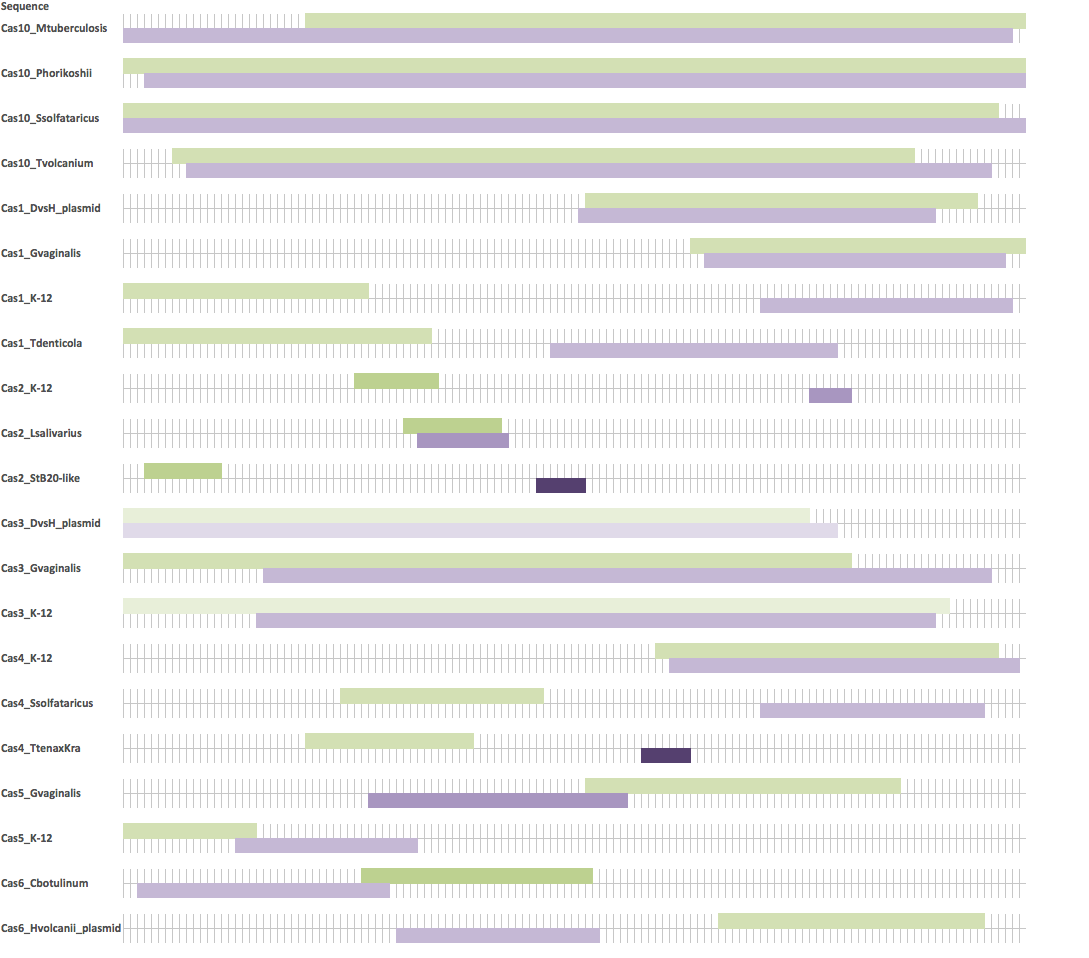
\includegraphics[scale = 0.45]{images/dp_figure1}
      \caption{Pairwise sequence alignment of various \textit{Cas} protein sequences against \textit{s. pyogenes Cas9} protein sequence. Green bars show coverage of semi-global alignment of individual sequence against \textit{s. pyogenes Cas9}. Purple bars show coverage of local alignment of individual sequence against \textit{s. pyogenes Cas9}. Darker color indicates higher average score per base, and therefore higher sequence similarity. Each grey marker represents 10 amino acid residues}
      \label{dp1}
\end{figure}

\begin{figure}[ht]
  \centering
  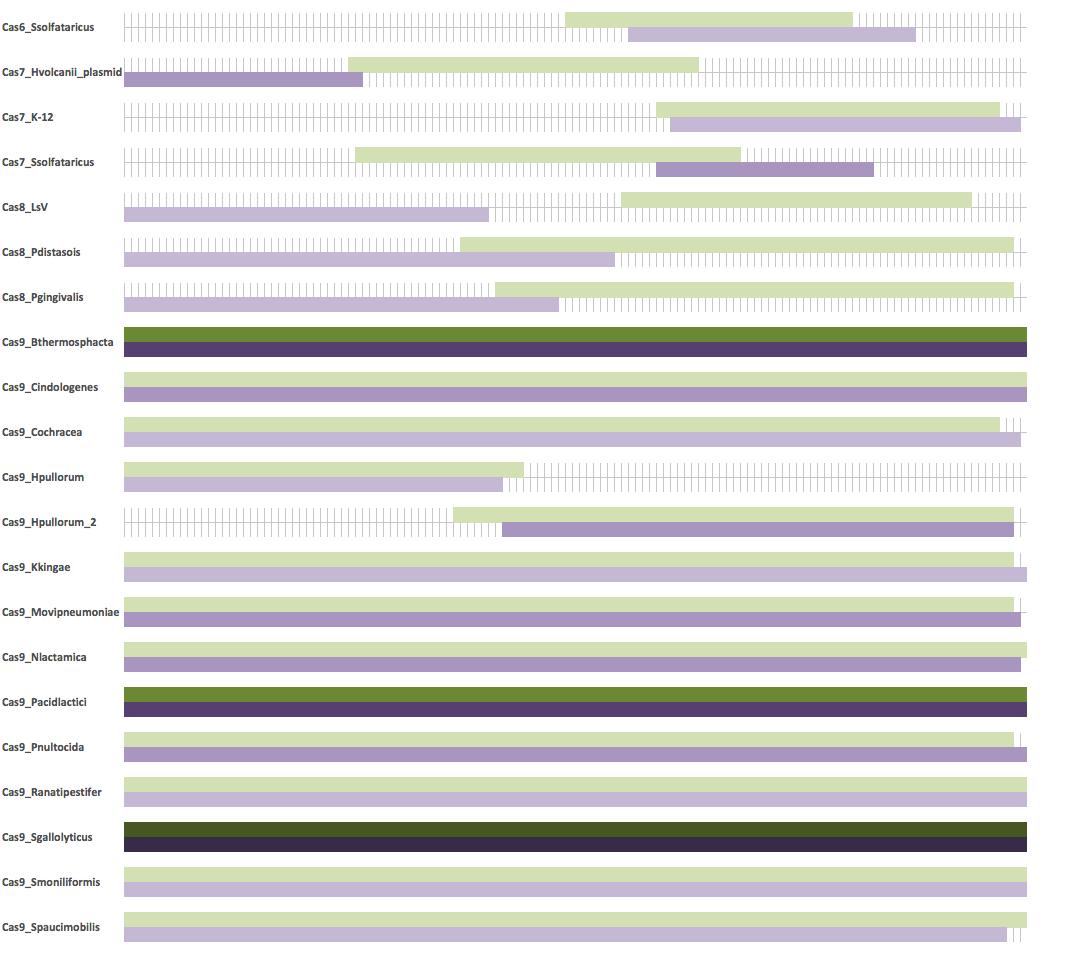
\includegraphics[scale = 0.45]{images/dp_figure2}
      \caption{Pairwise sequence alignment of various \textit{Cas} protein sequences against \textit{s. pyogenes Cas9} protein sequence. Green bars show coverage of semi-global alignment of individual sequence against \textit{s. pyogenes Cas9}. Purple bars show coverage of local alignment of individual sequence against \textit{s. pyogenes Cas9}. Darker color indicates higher average score per base, and therefore higher sequence similarity. Each grey marker represents 10 amino acid residues}
      \label{dp2}
\end{figure}

\subsection{Gibbs Sampling}

\subsubsection{Proof of concept}

The simulated sequences contain a motif with length 16 at various locations in the set of sequences and the sequences in the set contain either this motif or this motif and another motif shared by half some of the sequences (see \Cref{fig:design}). We trained motif with lengths 5, 10, 15, 16 (the correct length), 20, and 30. The results are shown in \Cref{fig:proof}. It shows that our strategy can successfully recognize and recover the position of the conserved region. And furthermore, as the motif length matches exactly the underlying truth, the number of outliers is minimized and if the length is close enough or slightly longer than the truth, the method is still robust. From the accuracy perspective, also, the accuracy is minimized if we use the right width but if the width is chosen within an appropriate range, then the true position is roughly within 10 amino acids to the predicted ones, which is still acceptable for our goal.

Besides, simulated data, the similar analysis was done using globin data as well. We performed the analysis using width 10, 30, 50, ..., 130. \Cref{fig:recog} shows the results of pattern recognition using learned motif with width 10, 50, 110, where we learned 10 motifs with width 10 and 5 for others. Here the score in each cell is defined as the maximum score among all the scores obtained by any possible window such position evolving with any motifs learned. It turns out that our method can find the conserved region at test time even though the motif is short, which implies that our method has enough sensitivity for our task.
\begin{figure}
  \centering
  \begin{minipage}{0.8\textwidth} % choose width suitably
  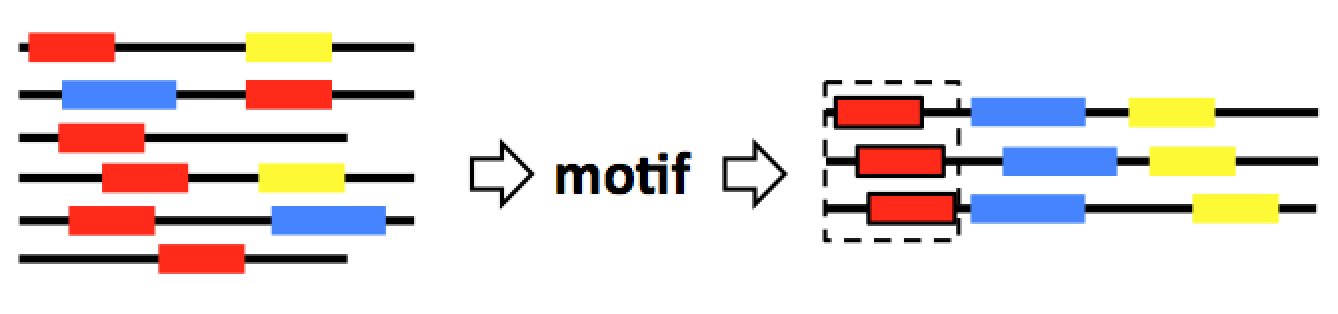
\includegraphics[width=\textwidth]{images/chart}
  {\footnotesize Simulated data has three motifs and every sequence at training time share the same motif (red) but may or may not contain other motifs (yellow/blue). At test time, the sequences share similar pattern and we chech if the trained motif can successfully recover the shared pattern (red).\par}
  \end{minipage}
  \caption{Gibbs sampling approach - The overview of the analysis design for simulated data}
  \label{fig:design}
\end{figure}

\begin{figure}[htbp]
  \centering
  \begin{minipage}{0.32\textwidth}
    \centering
    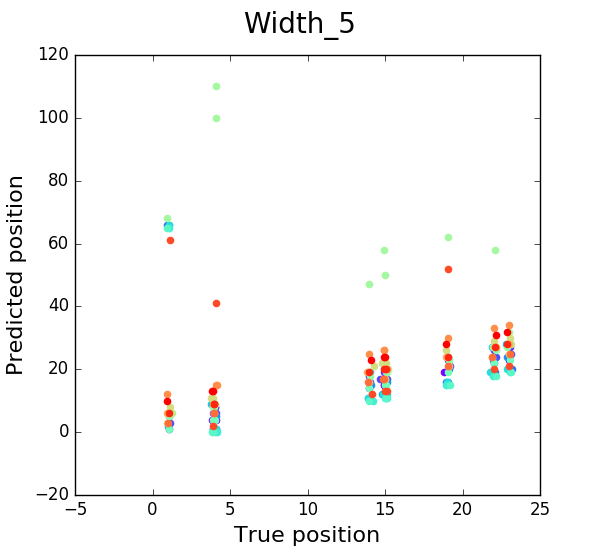
\includegraphics[width=1\textwidth]{images/Width_5} % first figure itself
    % \caption{first figure}
  \end{minipage}
  \hfill
  \begin{minipage}{0.32\textwidth}
    \centering
    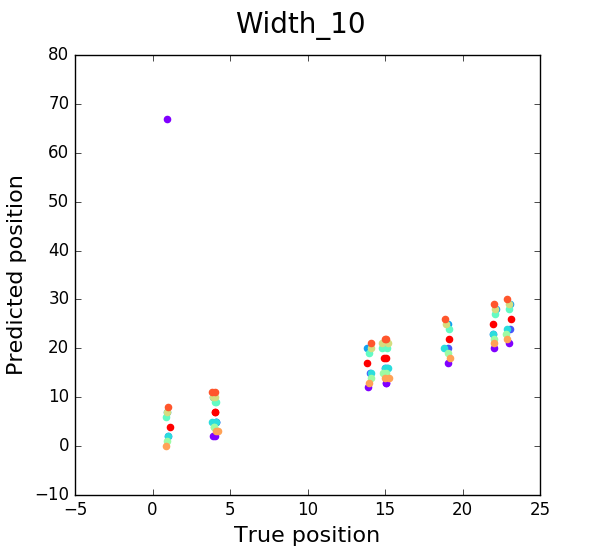
\includegraphics[width=1\textwidth]{images/Width_10} % second figure itself
    % \caption{second figure}
  \end{minipage}
  \hfill
  \begin{minipage}{0.32\textwidth}
    \centering
    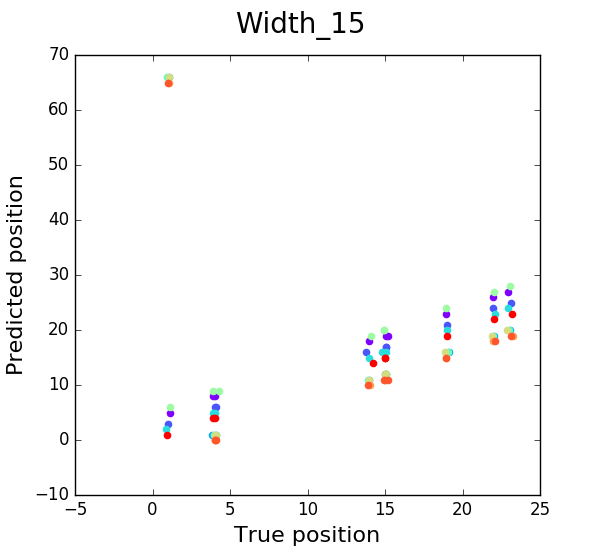
\includegraphics[width=1\textwidth]{images/Width_15} % second figure itself
    % \caption{second figure}
  \end{minipage}
  \vfill
  \begin{minipage}{0.32\textwidth}
    \centering
    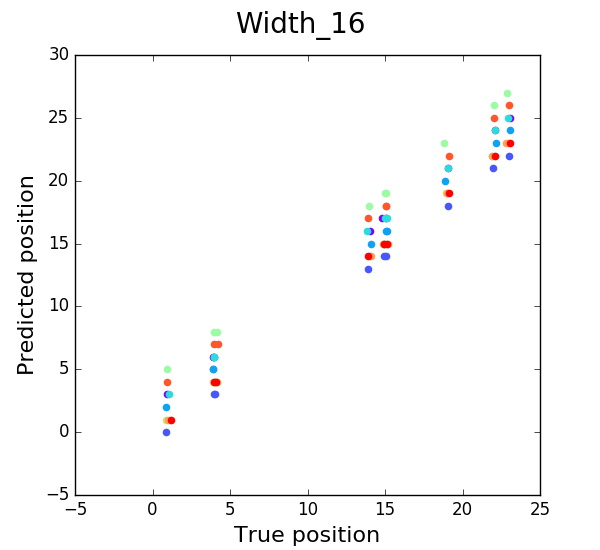
\includegraphics[width=\textwidth]{images/Width_16} % first figure itself
    % \caption{first figure}
  \end{minipage}
  \hfill
  \begin{minipage}{0.32\textwidth}
    \centering
    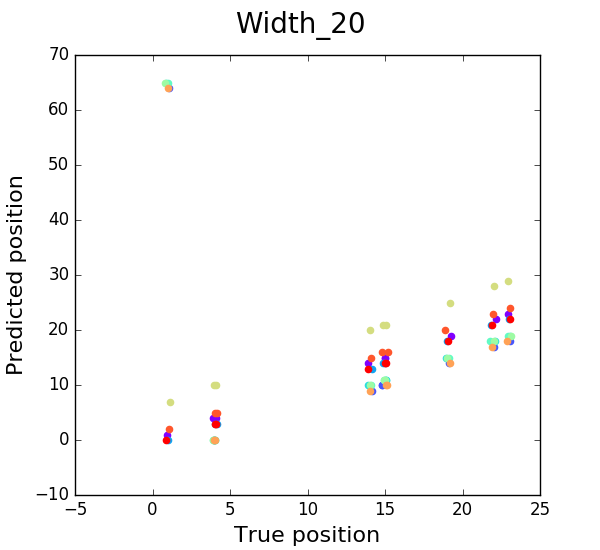
\includegraphics[width=\textwidth]{images/Width_20} % second figure itself
    % \caption{second figure}
  \end{minipage}
  \hfill
  \begin{minipage}{0.32\textwidth}
    \centering
    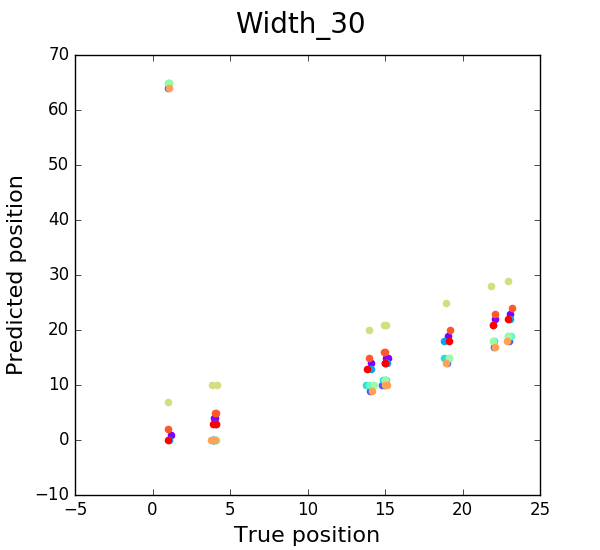
\includegraphics[width=\textwidth]{images/Width_30} % second figure itself
    % \caption{second figure}
  \end{minipage}
  \caption{Gibbs sampling approach - The results of conserved region finding in simulated sequences}
  \label{fig:proof}
\end{figure}

\begin{figure}[htbp]
  \centering
  \begin{minipage}{0.32\textwidth}
    \centering
    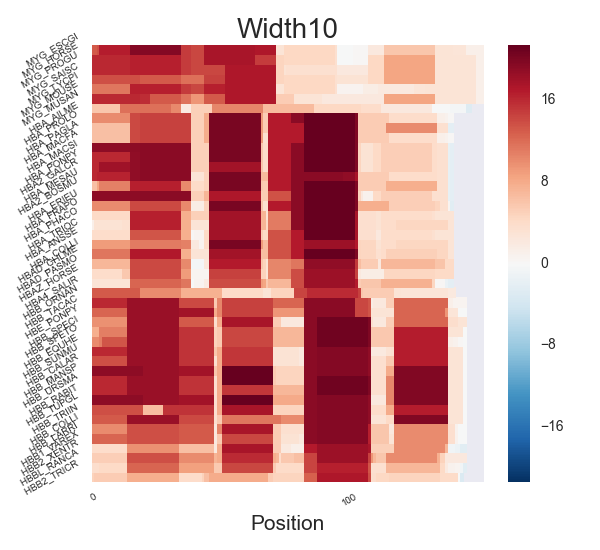
\includegraphics[width=1\textwidth]{images/Width10_heatmap} % first figure itself
    % \caption*{first figure}
  \end{minipage}
  \hfill
  \begin{minipage}{0.32\textwidth}
    \centering
    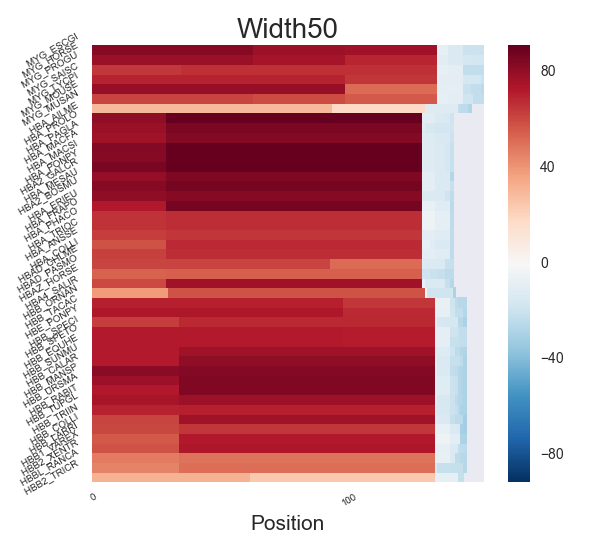
\includegraphics[width=1\textwidth]{images/Width50_heatmap} % second figure itself
    % \caption*{second figure}
  \end{minipage}
  \hfill
  \begin{minipage}{0.32\textwidth}
    \centering
    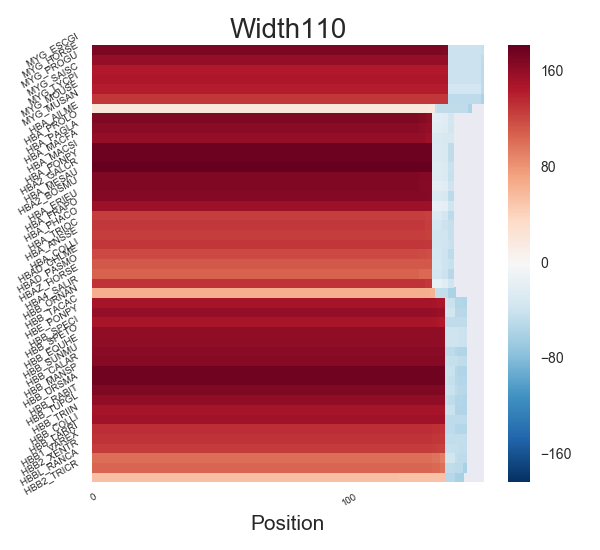
\includegraphics[width=1\textwidth]{images/Width110_heatmap} % second figure itself
    % \caption*{second figure}
  \end{minipage}
  \caption{Gibbs sampling approach - The pattern recognition scores of globins}
  \label{fig:recog}
\end{figure}

\subsubsection{Motif finding in Cas5 and Cas7}

The optimization curves of motif finding in Cas5 and Cas7 with width 10, 50, 110 are shown in \Cref{fig:cas5} and \Cref{fig:cas7}. From the curves we can see the Markov chain almost converges in each run.
\begin{figure}[htbp]
  \centering
  \begin{minipage}{0.32\textwidth}
    \centering
    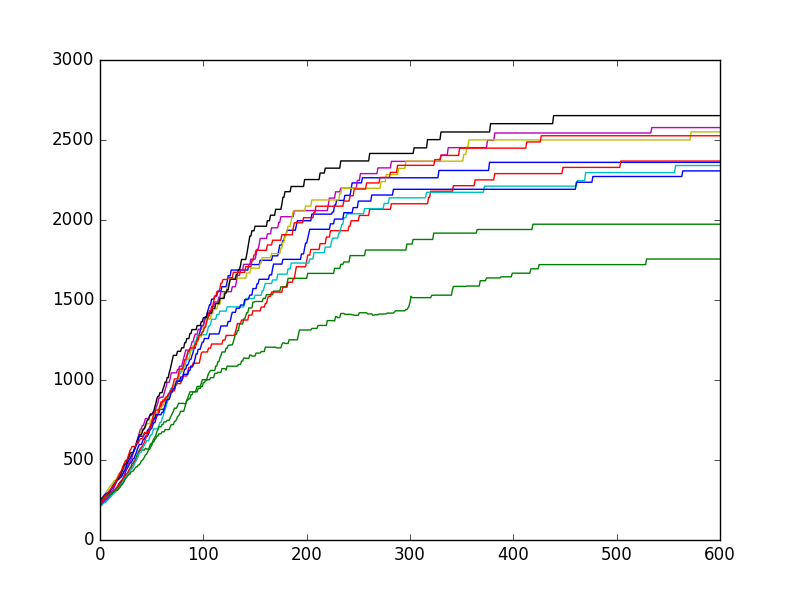
\includegraphics[width=1\textwidth]{images/cas5_width10_curve} % first figure itself
    \caption*{Width = 10}
  \end{minipage}
  \hfill
  \begin{minipage}{0.32\textwidth}
    \centering
    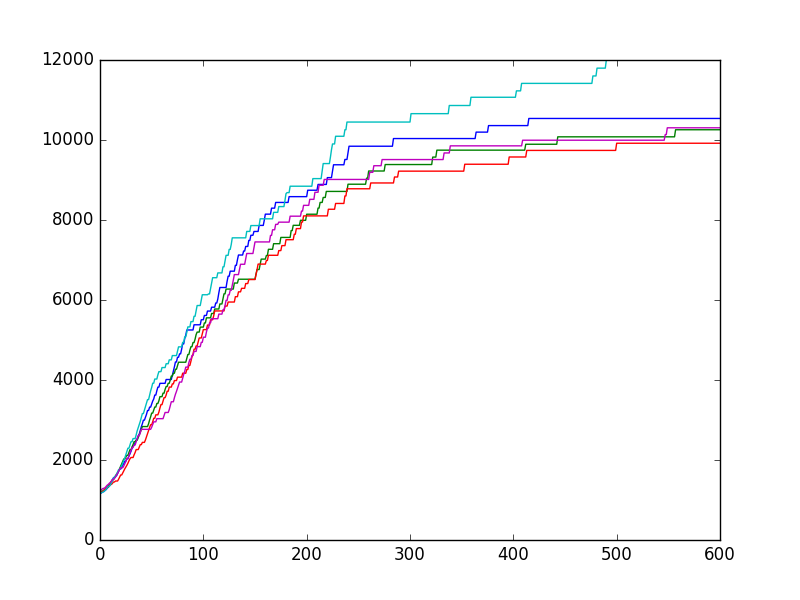
\includegraphics[width=1\textwidth]{images/cas5_width50_curve} % second figure itself
    \caption*{Width = 50}
  \end{minipage}
  \hfill
  \begin{minipage}{0.32\textwidth}
    \centering
    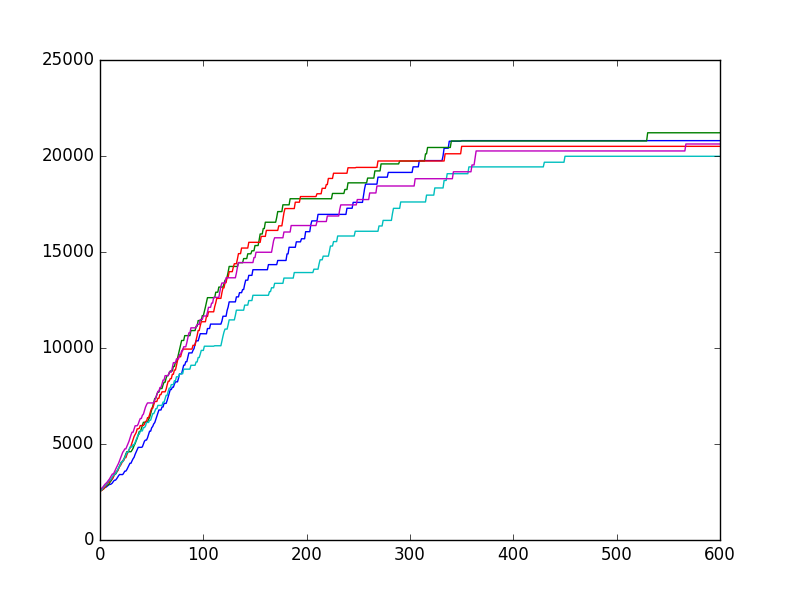
\includegraphics[width=1\textwidth]{images/cas5_width110_curve} % second figure itself
    \caption*{Width = 110}
  \end{minipage}
  \caption{Gibbs sampling approach - The optimization curves for motif finding in Cas5}
  \label{fig:cas5}
\end{figure}

\begin{figure}[htbp]
  \centering
  \begin{minipage}{0.32\textwidth}
    \centering
    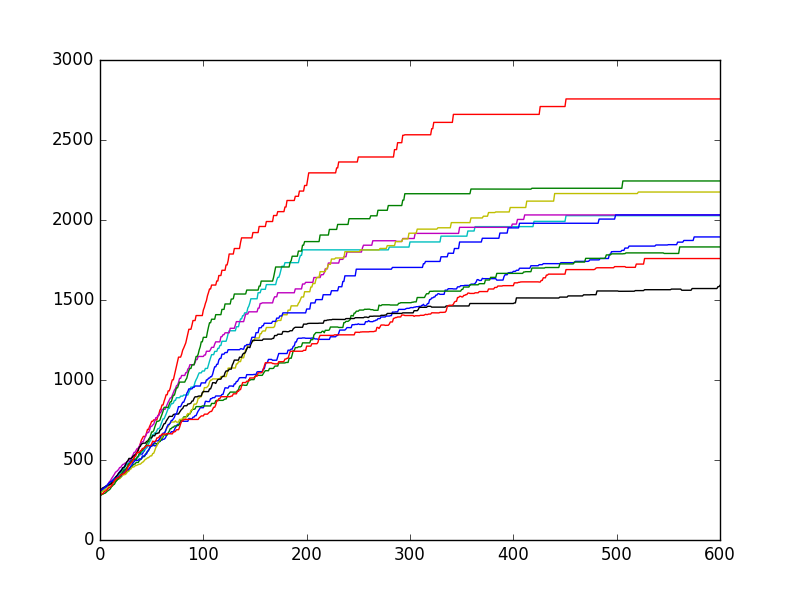
\includegraphics[width=1\textwidth]{images/cas7_width10_curve} % first figure itself
    \caption*{Width = 10}
  \end{minipage}
  \hfill
  \begin{minipage}{0.32\textwidth}
    \centering
    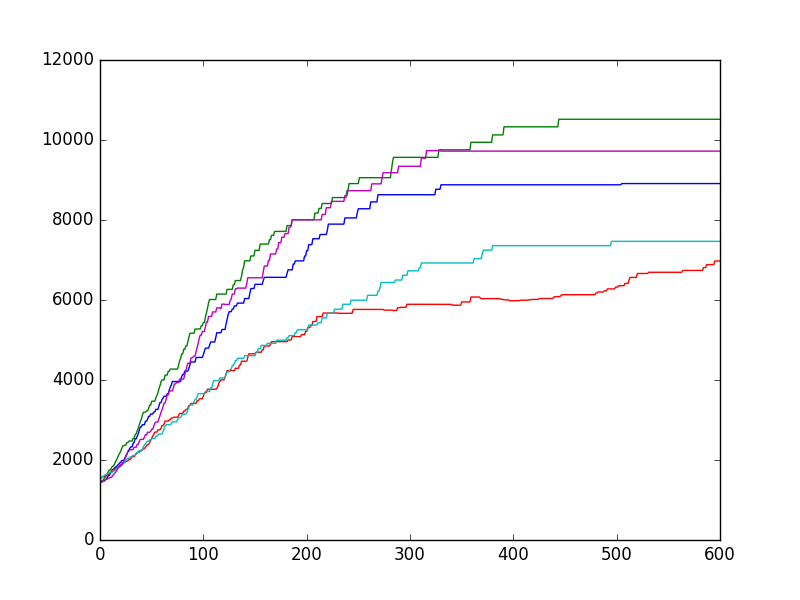
\includegraphics[width=1\textwidth]{images/cas7_width50_curve} % second figure itself
    \caption*{Width = 50}
  \end{minipage}
  \hfill
  \begin{minipage}{0.32\textwidth}
    \centering
    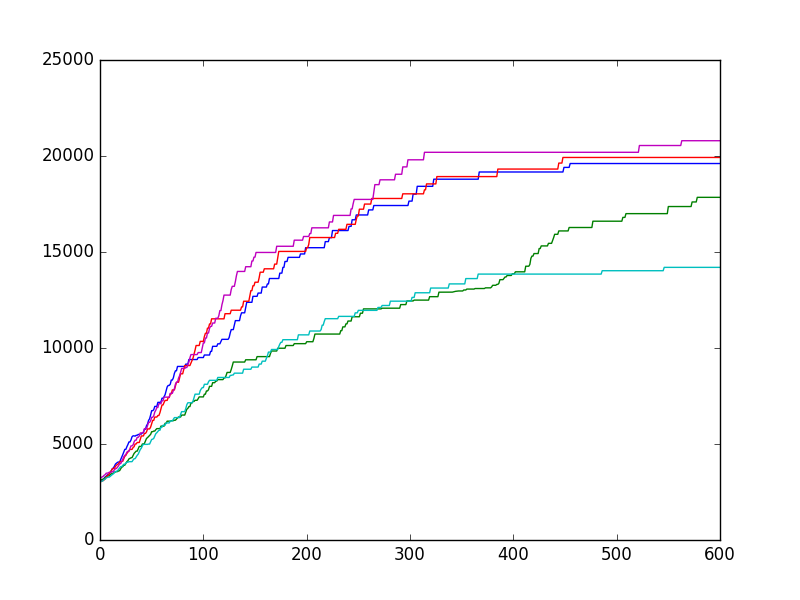
\includegraphics[width=1\textwidth]{images/cas7_width110_curve} % second figure itself
    \caption*{Width = 110}
  \end{minipage}
  \caption{Gibbs sampling approach - The optimization curves for motif finding in Cas7}
  \label{fig:cas7}
\end{figure}

\subsubsection{Pattern recognition in Cas9}

The results of pattern recognitions are shown in \Cref{fig:cas5_recog} and \Cref{fig:cas7_recog}. It turns out that for motif with width 10, we some noises and for motif with width 50 and 110, we get no single at all.

\begin{figure}[htbp]
  \centering
  \begin{minipage}{0.32\textwidth}
    \centering
    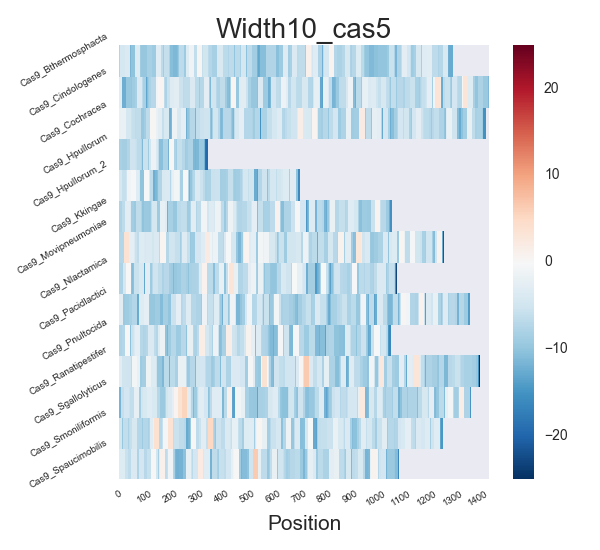
\includegraphics[width=1\textwidth]{images/Width10_cas5_heatmap} % first figure itself
    % \caption*{Width = 10}
  \end{minipage}
  \hfill
  \begin{minipage}{0.32\textwidth}
    \centering
    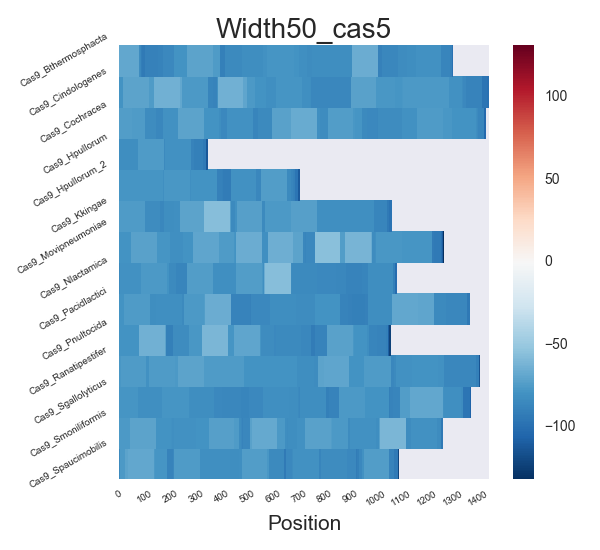
\includegraphics[width=1\textwidth]{images/Width50_cas5_heatmap} % second figure itself
    % \caption*{Width = 50}
  \end{minipage}
  \hfill
  \begin{minipage}{0.32\textwidth}
    \centering
    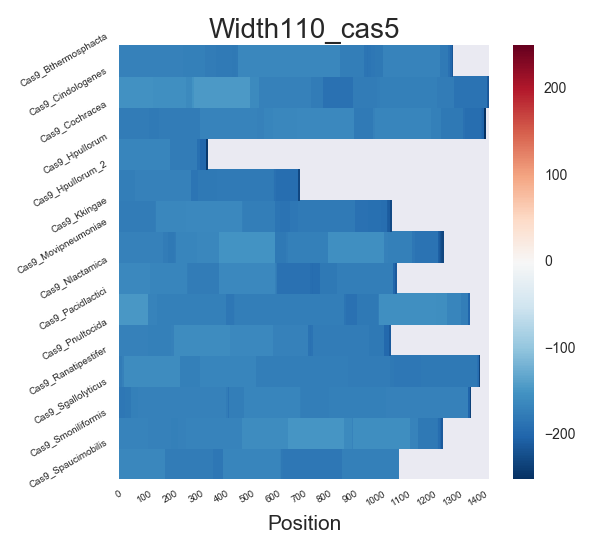
\includegraphics[width=1\textwidth]{images/Width110_cas5_heatmap} % second figure itself
    % \caption*{Width = 110}
  \end{minipage}
  \caption{Gibbs sampling approach - The pattern recognition scores of Cas9 with motifs found in Cas5}
  \label{fig:cas5_recog}
\end{figure}

\begin{figure}[htbp]
  \centering
  \begin{minipage}{0.32\textwidth}
    \centering
    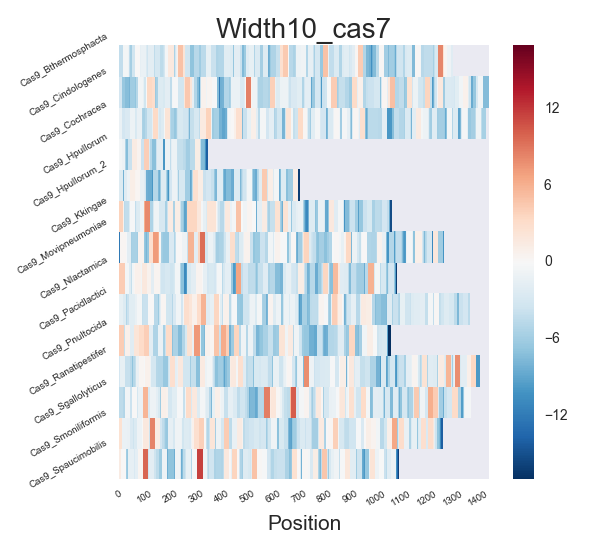
\includegraphics[width=1\textwidth]{images/Width10_cas7_heatmap} % first figure itself
    % \caption*{Width = 10}
  \end{minipage}
  \hfill
  \begin{minipage}{0.32\textwidth}
    \centering
    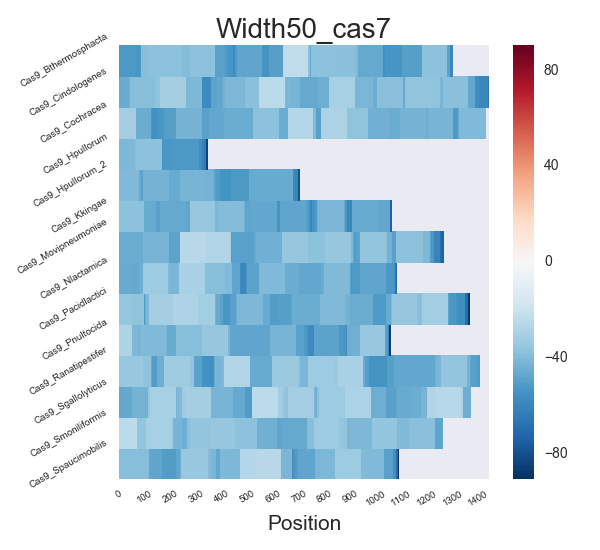
\includegraphics[width=1\textwidth]{images/Width50_cas7_heatmap} % second figure itself
    % \caption*{Width = 50}
  \end{minipage}
  \hfill
  \begin{minipage}{0.32\textwidth}
    \centering
    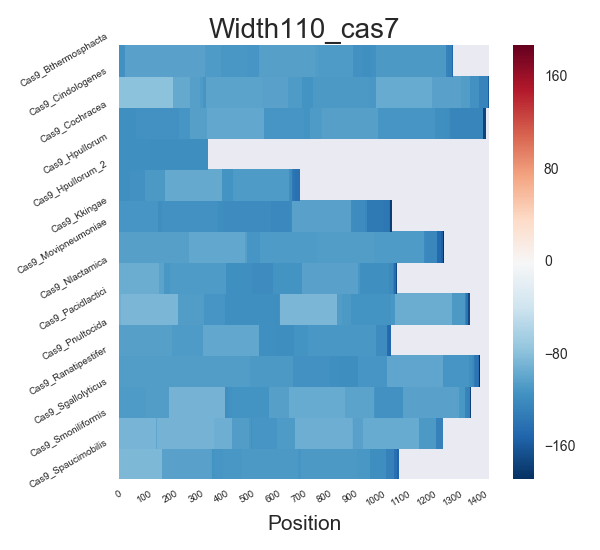
\includegraphics[width=1\textwidth]{images/Width110_cas7_heatmap} % second figure itself
    % \caption*{Width = 110}
  \end{minipage}
  \caption{Gibbs sampling approach - The pattern recognition scores of Cas9 with motifs found in Cas7}
  \label{fig:cas7_recog}
\end{figure}


\subsection{Domain-specific profile HMM}

\subsubsection{Protocol testing}

For method quality control purpose, some protocol was applied to globins4.fasta (a file of 4 sequences of globins generated from a tutorial file of HMMer). We built the profile Hmm and save it in golbins4.hmm. Using this profile HMM, we searched globins45.fa (a tutorial file of HMMer) and the result is saved into golbins.search. The summary of found domains is in the header part of the file as shown in Figure. \ref{hmm_test1}.  An example alignment of the found domain is shown in Figure. \ref{hmm_test2}. We can see that a domain is found in HBB\_MANSP. The profile HMM model can also be read from the alignment. Full result is available in golbins.search file.

\begin{figure}[ht]
  \centering
  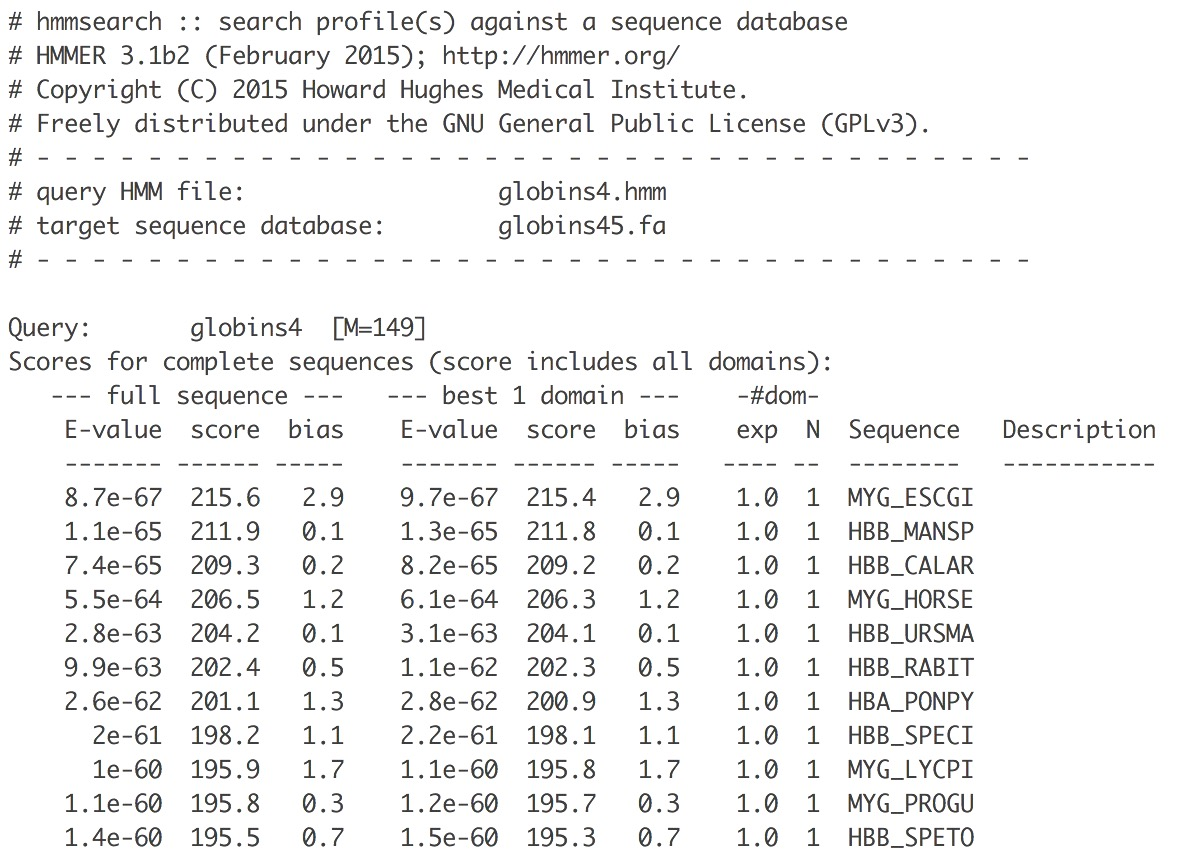
\includegraphics[scale = 0.35]{images/hmm_test1}
      \caption{profile HMM search results summary in globins.search}
      \label{hmm_test1}
\end{figure} 

\begin{figure}[ht]
  \centering
  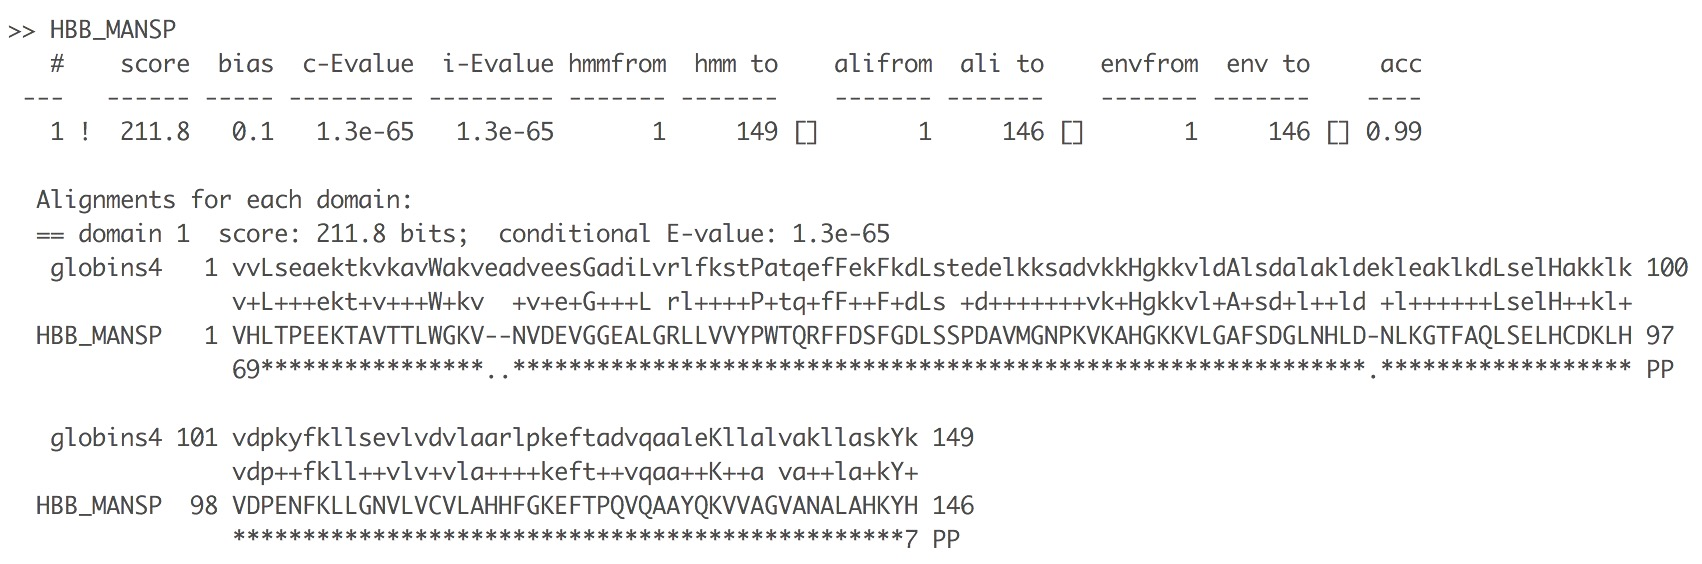
\includegraphics[scale = 0.3]{images/hmm_test2}
      \caption{profile HMM approach -  Domain alignment in globins.search}
      \label{hmm_test2}
\end{figure} 


\subsubsection{Finding domains of \textit{Cas9}}

After subtracting and aligning all the shared domains of \textit{Cas9} marked in EMBL-EBI. We built profile HMMs from these multi-sequence alignments and save them into data/domains\_Cas9/IPR032239.hmm, etc. Then we use these models to find the domains of \textit{Cas9} in all \textit{Cas} family protein sequences, hoping to find similar domains in other proteins in different subtypes. The summary of one of the search results can be seen in Figure. \ref{Cas9}. The profile HMM can find similar domains in other \textit{Cas9} proteins, which is as expected. But all the models failed to find any similar domains in other \textit{Cas} family proteins other than \textit{Cas9}.

\begin{figure}[ht]
  \centering
  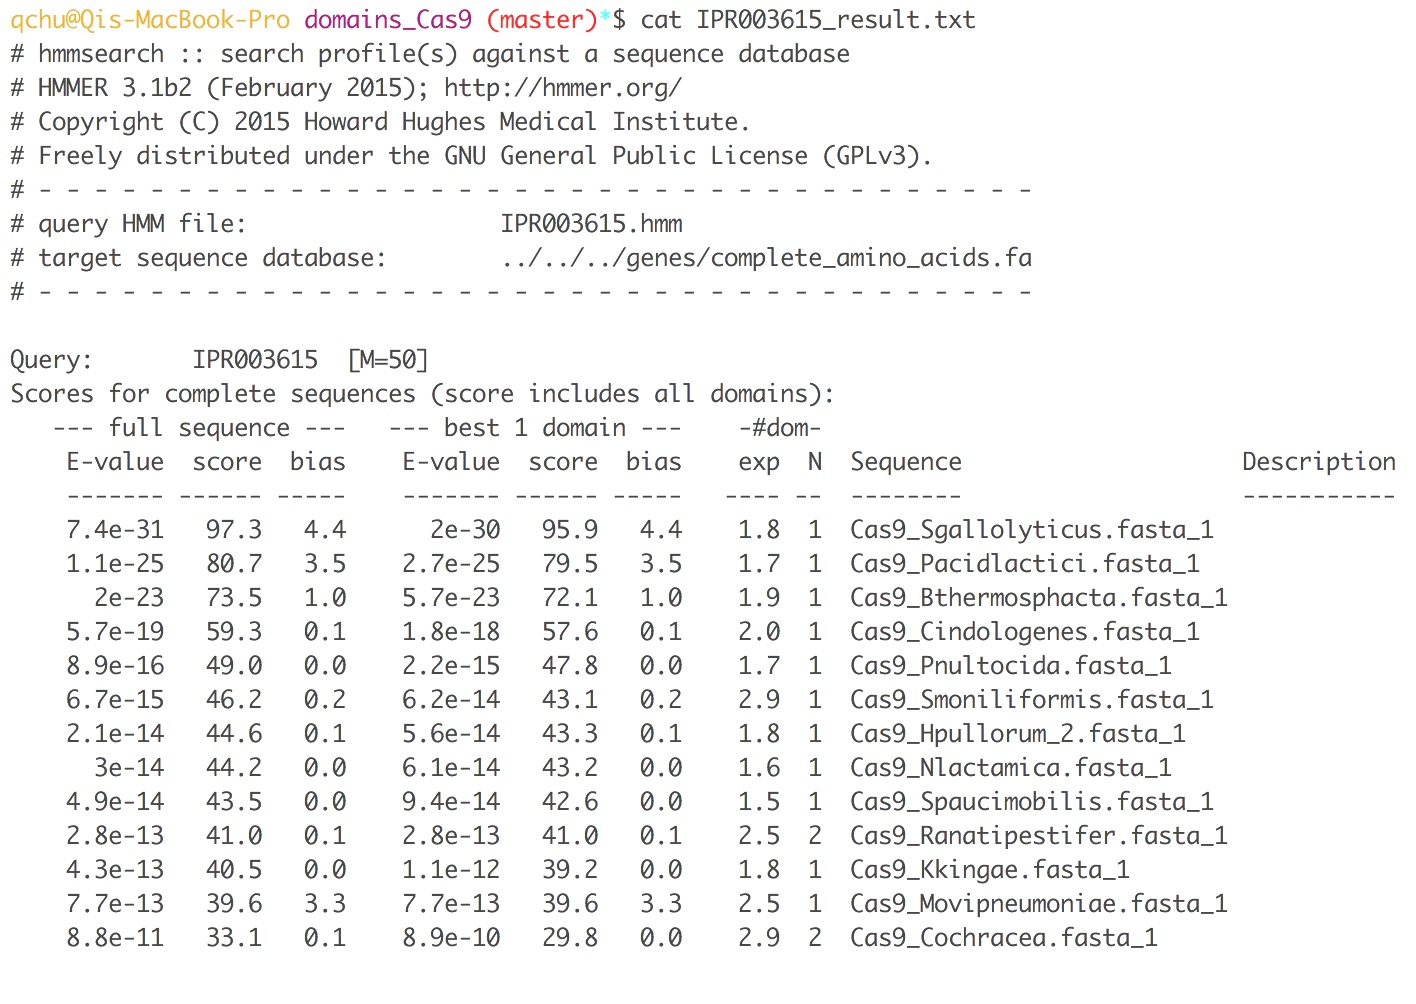
\includegraphics[scale = 0.3]{images/cas9Domain}
      \caption{profile HMM approach - One example result for searching for \textit{Cas9} in all \textit{Cas} family proteins}
      \label{Cas9}
\end{figure} 

\subsection{Finding domains of \textit{Cas5}}

We also tried the other direction. That is to use domain markers of \textit{Cas5}, which is a component of Type I system, and to find similar domains in \textit{Cas9}. The protocol is the same and one of the summaries of the results can be found in Figure \ref{Cas5}. The result is similar, the model is able to find some similar domains in other \textit{Cas5} proteins but not other \textit{Cas} family proteins.

\begin{figure}[ht]
  \centering
  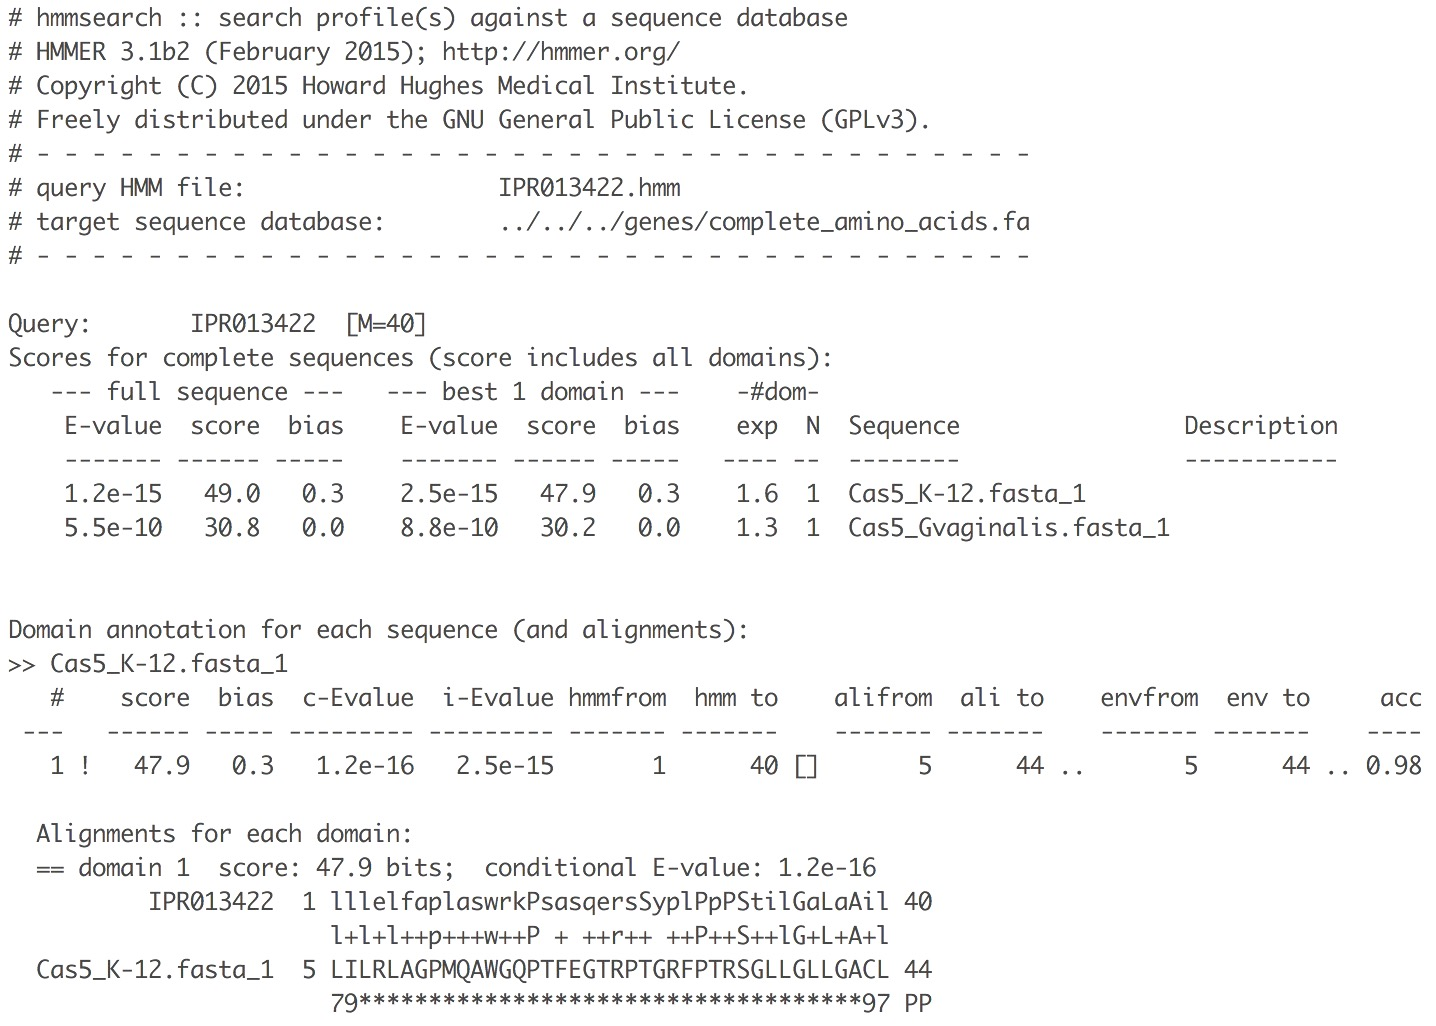
\includegraphics[scale = 0.3]{images/cas5Domain}
      \caption{profile HMM approach - One example result for searching for \textit{Cas5} in all \textit{Cas} family proteins}
      \label{Cas5}
\end{figure} 

\section{Conclusion}

In sequence alignment model, successful mapping of various \textit{Cas9} protein to \textit{Cas9} was observed to depend on the length of the query sequence. \textit{Cas10}, the biggest protein in CRISPR Class 1, mapped to \textit{Cas9} most accurately in both local and semi-global alignment. What was interesting is how much of \textit{Cas1, Cas2} and \textit{Cas4} mapped to \textit{Cas9}, despite the fact these three proteins are part of adaption functionality rather than interference functionality\cite{cas:makarova}. Another example of both local alignment and semiglobal alignment successfully mapping is \textit{Cas9} sequence of \textit{Helicobacter pullorum}, where the \textit{Cas9} that has been split into two parts, mapped neatly to the \textit{s.pyogenes Cas9}. In this alignment, difference in the semiglobal(green in figure\ref{dp2}) and local(purple in figure\ref{dp2}) alignment show the actual conserved regions in purple, and the regions of semiglobal alignment that does not have corresponding local alignment would indicate some extraneous sequence at either ends of the protein. 


However, in some cases, local and global alignment disagreed as for where to map to in \textit{s.pyogenes Cas9}. One example would be \textit{Cas8}, where all three sequences of \textit{Cas8} aligned disagreed on semiglobal vs local alignment. Given that both local alignment and semiglobal alignment were performed using the same substitution matrix (\texttt{BLOSUM62}) and same gap penalties with the only difference being except for end gap penalty and traceback startpoint, we would be more inclined to trust the local alignment in terms of motif-finding, because average score per position for such conflicting alignments is much higher for local alignment, and because it does not penalize overall sequence alignment for certain highly divergent regions within the gene. Default BLAST parameters, such as \texttt{BLOSUM62}, were used due to limited predictions currently available for accurate phylogenetic model of CRISPR family. These parameters have been shown to have the best performance overall when there is limited information about evolutionary distance and divergence. By modifying parameters to fit the actual evolutionary distance when such data is available (including, but not limited to substitution matrix, gap costs, etc.), much more accurate alignment and motif detection through sequence alignment could be obtained.




The Gibbs sampling model was verified to successfully identify conserved regions in simulated sequences and globin data, which indicates that the motif finding approach with PSSMs is capable of finding underlying conserved regions in sequences. However, the same motif finding approach fails in the analysis of \textit{Cas} protein family. The main reason is that the conserved region shared by Cas family might be evolutionarily far to divergent compared to the globin family and the signal is hard to be captured by the default PSSM without utilizing any molecular evolution information. Also, the size of our training data is small and it may prevent discovery of motifs in sequences that are divergent too divergent. This pitfall leads to the possibility that the discovered motifs might not be representative of the entire \textit{CRISPR} protein family, and might be too stringent and overfitted to particular input data. 




Profile-HMM was also verified to successfully identify conserved domains in the globin-family. In addition, it successfully identified the domains in the same subtype as the model source. For example, the model built from \textit{Cas9} can find most domains in \textit{Cas9} in other species. But it failed to find similar domains across different subtypes in the \textit{Cas} family. One possible reason for the failure is that the limited number of training sequences makes the model too rigid to be able to fit remotely related sequences. Another possible reason is that even though different proteins in different subtypes have similar functionalities, they evolved separately and have low level sequence similarity. 


Pairwise sequence alignment model implicitly incorporates biophysical properties while making alignment and motif predictions, but assumed sequence independence. Gibbs Sampling or HMM profiling do not take biophysical properties into consideration, but both consider multiple sequence for each position. Gibbs sampling is easy to implement and much more intuitive to understand and require relatively less data compared to HMM, but also assumed positional independence in evolution. HMM profiling addresses many of the features lacking in pairwise sequence alignment or Gibbs sampling, but generally requires much more data. However, there is finite number of \textit{Cas} sequences and even less in terms of actually available sequences. 


In case of Gibbs and HMM models, both were shown to accurately predict conserved regions with the control data : Globin family and simulated sequences. However, Globin proteins belong to eukaryotes whose evolutionary history is much shorter than that of the prokaryotes - bacteria and archaea - which possess the CRISPR system. It may be that these models as-is are too stringent for identifying evolutionary relationships and motifs in much more distant protein family than a highly conserved protein like globin, in a relatively short evolutionary timestep. Performance of all current methods for identifying similarities or motif finding decrease as evolutionary diversity and divergence of the protein family being studied increases. Much more work can and should be done in development of models specifically for studying and identifying the relationship and conservation of motifs among distantly related organisms. 


Our study has many potential directions it could take for improvement and expansions. One approach may be to increase our dataset to include even greater number of \textit{Cas} protein sequences. Also, all three models would greatly benefit from a more updated prediction of evolutionary timeline and relationship between the \textit{Cas} proteins for additional parameter tuning for more accurate motif discovery. Recall that the motif finding approach fails in the task with the potential lack of power in motif representation and the lack of data. One of the ways to overcome this pitfall is to reduce the size our alphabet. For example, instead of using the whole alphabet (20 amino acids), we can use 5-character alphabet where 5 characters indicate the biochemical properties of the residues. This can partly solve the problem of limited data by reducing the complexity of our model, and furthermore, it also automatically makes use of biochemical property and evolutionary 

\begin{thebibliography}{1}

\bibitem{cas:makarova}
K. S. ~Makarova, et al., \emph{An updated evolutionary classification of CRISPR-Cas systems}  \hskip 1em plus 0.5em minus 0.4em\relax http://dx.doi.org/10.1038/nrmicro3569, 28 September 2015

\bibitem{needlemanwunsch}
Saul B. Needleman, Christian D. Wunsch, \emph{A general method applicable to the search for similarities in the amino acid sequence of two proteins} \hskip 1em plus 0.5em minus 0.4em\relax http://www.sciencedirect.com/science/article/pii/0022283670900574, 28 March 1970

\bibitem{smithwaterman}
Smith, Temple F., Waterman, Michael S., \emph{Identification of Common Molecular Subsequences} \hskip 1em plus 0.5em minus 0.4em\relax Journal of Molecular Biology. 147: 195-197. doi:10.1016/0022-2836(81)90087-5. PMID 7265238., 1981

\bibitem{preWork}
Makarova, Kira S et al. ?Unification of Cas Protein Families and a Simple Scenario for the Origin and Evolution of CRISPR-Cas Systems.? Biology Direct 6 (2011): 38. PMC. Web. 26 Nov. 2016.

\bibitem{annualreview}
Devaki Bhaya,Michelle Davison, and Rodolphe Barrangou, \emph{CRISPR-Cas Systems in Bacteria and Archaea: Versatile Small RNAs for Adaptive Defense and Regulation} \hskip 1em plus 0.5em minus 0.4em\relax Annual Review of Genetics Vol. 45: 273-297 (Volume publication date December 2011) DOI: 10.1146/annurev-genet-110410-132430

\bibitem{mali}
Mali, P., Esvelt, K. M., \& Church, G. M. (2013). Cas9 as a versatile tool for engineering biology. Nature Methods, 10(10), 957?963. doi:10.1038/nmeth.2649

\bibitem{jenniferdoudna}
Jinek M, Chylinski K, Fonfara I, Hauer M, Doudna JA, Charpentier E., \emph{A programmable dual-RNA-guided DNA endonuclease in adaptive bacterial immunity} \hskip 1em plus 0.5em minus 0.4em\relax Science. 2012 Aug 17;337(6096):816-21. doi: 10.1126/science.1225829. Epub 2012 Jun 28.

\bibitem{fengzhang}
Ran, F Ann and Hsu, Patrick D and Wright, Jason and Agarwala, Vineeta and Scott, David A and Zhang, Feng, \emph{Genome engineering using the CRISPR-Cas9 system} \hskip 1em plus 0.5em minus 0.4em\relax Nat. Protocols(2013) http://dx.doi.org/10.1038/nprot.2013.143

\bibitem{stanleyqi}
Qi LS, Larson MH, Gilbert LA, Doudna JA, Weissman JS, Arkin AP, Lim WA., \emph{Repurposing CRISPR as an RNA-guided platform for sequence-specific control of gene expression} \hskip 1em plus 0.5em minus 0.4em\relax Cell. 2013 Feb 28;152(5):1173-83. doi: 10.1016/j.cell.2013.02.022.


\bibitem{cas9structure}
Hiroshi Nishimasu, F. Ann Ran, Patrick D. Hsu, Silvana Konermann, Soraya I. Shehata, Naoshi Dohmae, Ryuichiro Ishitani, Feng Zhang, Osamu Nureki \emph{Crystal Structure of Cas9 in Complex with Guide RNA and Target DNA} http://www.cell.com/cell/pdf/S0092-8674(14)00156-1.pdf February 13, 2014

\bibitem{doublenick}
Ran FA, Hsu PD, Lin C-Y, et al. \emph{Double nicking by RNA-guided CRISPR Cas9 for enhanced genome editing specificity.} Cell. 2013;154(6):1380-1389. doi:10.1016/j.cell.2013.08.021.

\bibitem{aav1}
Ran FA,  et al., \emph{In vivo genome editing using Staphylococcus aureus Cas9} Nature 520, 186?191 (09 April 2015) doi:10.1038/nature14299

\bibitem{aav2}
I. Maggio et al., \emph{Adenoviral vector delivery of RNA-guided CRISPR/Cas9 nuclease complexes induces targeted mutagenesis in a diverse array of human cells} Scientific Reports 4, Article number: 5105 (2014) doi:10.1038/srep05105


\bibitem{hmmer}
HMMER 3.1b2 (February 2015); http://hmmer.org/

\bibitem{stormo1982use}
G.~D. Stormo, T.~D. Schneider, L.~Gold, and A.~Ehrenfeucht, ``Use of the
  ‘perceptron’algorithm to distinguish translational initiation sites in e.
  coli,'' {\em Nucleic Acids Research}, vol.~10, no.~9, pp.~2997--3011, 1982.

\bibitem{lawrence1993detecting}
C.~E. Lawrence, S.~F. Altschul, M.~S. Boguski, J.~S. Liu, A.~F. Neuwald, J.~C.
  Wootton, {\em et~al.}, ``Detecting subtle sequence signals: a gibbs sampling
  strategy for multiple alignment,'' {\em SCIENCE-NEW YORK THEN WASHINGTON-},
  vol.~262, pp.~208--208, 1993.

\end{thebibliography}

% \bibliography{gibbs_sampler}{}
% \bibliographystyle{ieeetr}

\end{document}


